% Options for packages loaded elsewhere

\PassOptionsToPackage{unicode}{hyperref}

\PassOptionsToPackage{hyphens}{url}

%

\documentclass[

  12pt,

  dutch,

  a4paper,

]{report}

\usepackage{lmodern}

\usepackage{amssymb,amsmath}

\usepackage{ifxetex,ifluatex}

\ifnum 0\ifxetex 1\fi\ifluatex 1\fi=0 % if pdftex

  \usepackage[T1]{fontenc}

  \usepackage[utf8]{inputenc}

  \usepackage{textcomp} % provide euro and other symbols

\else % if luatex or xetex

  \usepackage{unicode-math}

  \defaultfontfeatures{Scale=MatchLowercase}

  \defaultfontfeatures[\rmfamily]{Ligatures=TeX,Scale=1}

\fi

% Use upquote if available, for straight quotes in verbatim environments

\IfFileExists{upquote.sty}{\usepackage{upquote}}{}

\IfFileExists{microtype.sty}{% use microtype if available

  \usepackage[]{microtype}

  \UseMicrotypeSet[protrusion]{basicmath} % disable protrusion for tt fonts

}{}

\makeatletter

\@ifundefined{KOMAClassName}{% if non-KOMA class

  \IfFileExists{parskip.sty}{%

    \usepackage{parskip}

  }{% else

    \setlength{\parindent}{0pt}

    \setlength{\parskip}{6pt plus 2pt minus 1pt}}

}{% if KOMA class

  \KOMAoptions{parskip=half}}

\makeatother

\usepackage{xcolor}

\IfFileExists{xurl.sty}{\usepackage{xurl}}{} % add URL line breaks if available

\IfFileExists{bookmark.sty}{\usepackage{bookmark}}{\usepackage{hyperref}}

\hypersetup{

  pdftitle={Functioneel Ontwerp van ‘Big’},

  pdfauthor={Gerard Edelaar},

  pdflang={nl-NL},

  hidelinks,

  pdfcreator={LaTeX via pandoc}}

\urlstyle{same} % disable monospaced font for URLs

\usepackage{longtable,booktabs}

% Correct order of tables after \paragraph or \subparagraph

\usepackage{etoolbox}

\makeatletter

\patchcmd\longtable{\par}{\if@noskipsec\mbox{}\fi\par}{}{}

\makeatother

% Allow footnotes in longtable head/foot

\IfFileExists{footnotehyper.sty}{\usepackage{footnotehyper}}{\usepackage{footnote}}

\makesavenoteenv{longtable}

\usepackage{graphicx}

\makeatletter

\def\maxwidth{\ifdim\Gin@nat@width>\linewidth\linewidth\else\Gin@nat@width\fi}

\def\maxheight{\ifdim\Gin@nat@height>\textheight\textheight\else\Gin@nat@height\fi}

\makeatother

% Scale images if necessary, so that they will not overflow the page

% margins by default, and it is still possible to overwrite the defaults

% using explicit options in \includegraphics[width, height, ...]{}

\setkeys{Gin}{width=\maxwidth,height=\maxheight,keepaspectratio}

% Set default figure placement to htbp

\makeatletter

\def\fps@figure{htbp}

\makeatother

\setlength{\emergencystretch}{3em} % prevent overfull lines

\providecommand{\tightlist}{%

  \setlength{\itemsep}{0pt}\setlength{\parskip}{0pt}}

\setcounter{secnumdepth}{5}

% ============Ampersand specific Begin=================
% First a couple of LaTeX packages are included:

% The glossaries package supports acronyms and multiple glossaries
\usepackage[toc]{glossaries}    % Add the glossaries to the table of contents
% \makeglossaries

% geometry provides a flexible and easy interface to page dimentions
\usepackage[ top=1.5cm, bottom=1.5cm, outer=5cm, inner=2cm
            , heightrounded, footskip=.5cm
            , marginparwidth=2.5cm, marginparsep=0.5cm]{geometry}

% breqn – Automatic line breaking of displayed equations
\usepackage{breqn}

% colonequals – Colon equals symbols
\usepackage{colonequals}

% caption – Customising captions in floating environments
\usepackage{caption}
\captionsetup{format=plain
              ,textfont=bf,labelfont=small
              ,labelsep=none
              ,labelformat=empty
              ,width=.85\textwidth
              }

% textcomp – LATEX support for the Text Companion fonts -- Disabled because obsolete.
% \usepackage{textcomp}

% hypcap – Adjusting the anchors of captions
\usepackage[all]{hypcap}

% <Adaptation>: The LaTeX commands \[ and \], are redefined in the amsmath package, making sure that equations are
% not numbered. This is undesireable behaviour. this is fixed with the following hack, inspired on a note
% found at http://tex.stackexchange.com/questions/40492/what-are-the-differences-between-align-equation-and-displaymath
\DeclareRobustCommand{\[}{\begin{equation}}
\DeclareRobustCommand{\]}{\end{equation}}
% <End-adaptation>


% ============Ampersand specific End===================


\ifxetex

  % Load polyglossia as late as possible: uses bidi with RTL langages (e.g. Hebrew, Arabic)

  \usepackage{polyglossia}

  \setmainlanguage[]{dutch}

\else

  \usepackage[shorthands=off,main=dutch]{babel}

\fi



\title{Functioneel Ontwerp van Big}

\author{Gerard Edelaar}

\date{3 december 2021}



\begin{document}

\maketitle



{

\setcounter{tocdepth}{2}

\tableofcontents

}

\hypertarget{sec:Intro}{%
\chapter{Inleiding}\label{sec:Intro}}

\section{De wet BIG}

Het BIG-register is onderdeel van de Wet op de beroepen in de
individuele gezondheidszorg (BIG). Het doel van de Wet BIG is te zorgen
dat de kwaliteit van onze gezondheidszorg hoog is en blijft. Ook
beschermt de Wet BIG patiënten tegen ondeskundig en onzorgvuldig
handelen van zorgverleners.

De Wet BIG verdeelt beroepen die onder deze wet vallen in 3 groepen
volgens hun wettelijke artikelnummer: artikel 3-, 34- en artikel
36a-beroepen. In het BIG-register worden alleen artikel 3 en artikel
36a-beroepen geregistreerd. Daarnaast bestaan er ook wettelijk erkende
specialismen. Deze vallen onder artikel 14. Een specialisme wordt
aangetekend bij een artikel 3 beroep. Beroepen die in het BIG-register
staan geregistreerd vallen onder het tuchtrecht.

Naast het registreren en herregistreren van deze beroepsbeoefenaren en
de uitvoering van het tuchtrecht valt ook het erkennen van
(buitenlandse) diploma’s en onder de taken van het BIG-register.
Zorgverleners met een buitenlands diploma moeten voldoen aan de
Nederlandse opleidingseisen. Hun opleidingsniveau moet gelijk zijn aan
dat van een zorgverlener met een Nederlands diploma. Eventueel telt
relevante werkervaring mee om het niveau te bepalen. Het CIBG neemt
hierover een besluit op grond van het advies van de onafhankelijke
deskundigencommissie, de Commissie buitenslands gediplomeerden
volksgezondheid (CBGV).

Tevens kunnen zorgprofessionals bij het BIG-register terecht voor het
aanvragen van verklaringen en zorgt het bigregister voor het aantekenen
van specialismen en voorschrijfbevoegdheden.

Voor zorgconsumenten en organisaties biedt het BIG-register de
mogelijkheid te controleren of zijn zorgverlener bevoegd is om zijn of
haar beroep uit te oefenen.

\subsection{Opdrachtgever}

De Directie MEVA van het Ministerie van VWS is opdrachtgever voor de
uitvoering van de Wet BIG.

\subsection{Onderliggende wetgeving}

\begin{itemize}
\tightlist
\item
  \href{https://wetten.overheid.nl/BWBR0006251/2021-07-01}{Wet op de
  beroepen in de individuele gezondheidszorg}
\item
  \href{https://wetten.overheid.nl/BWBR0024841/2020-07-01}{Besluit
  periodieke registratie Wet BIG}
\item
  \href{https://wetten.overheid.nl/BWBR0007648/2021-01-01}{Registratiebesluit
  BIG}
\item
  \href{https://wetten.overheid.nl/BWBR0008688/2021-04-01}{Tuchtrechtbesluit
  BIG}
\item
  \href{https://wetten.overheid.nl/BWBR0025605/2020-12-15}{Regeling
  periodieke registratie Wet BIG}
\item
  \href{https://wetten.overheid.nl/BWBR0031720/2014-02-01}{Regeling
  tarieven registratie beroepsbeoefenaren Wet BIG}
\end{itemize}

Het BIGregister bevindt zich in een keten van informatieverstrekking en
is sterk afhankelijk van informatie van derden. Zo zijn derden weer
sterk afhankelijk van onze informatie.

\subsection{Huidig informatiesysteem}

De Wet BIG stamt uit 1993. Het huidige zaaksysteem (Zorro) is als
opvolger van Ribiz ontwikkeld in 2007. Eind 2018 is het eerste deel van
de publieke website vernieuwd. Medio 2019 volgt vernieuwing van een
volgend deel van de publieke website, waarmee op dat moment alleen de
advieswijzer nog niet is omgezet.

Dit document\footnote{Dit document is gegenereerd op 3-12-2021 om
  21:32:23, dmv. Ampersand-v4.6.0 {[}HEAD:743e5ce*{]}, build time:
  22-Nov-21 15:44:23 Coordinated Universal Time.} definieert de
functionaliteit van een informatiesysteem genaamd ‘Big’. Het definieert
de database en de business-services van Big door middel van
bedrijfsregels\footnote{Het ontwerpen met bedrijfsregels is een kenmerk
  van de Ampersand aanpak, die gebruikt is bij het samenstellen van dit
  document.}. Deze afspraken staan opgesomd in 2 , geordend op thema.

De diagnose in 3 is bedoeld voor de auteurs om gebreken uit hun
Ampersand model op te sporen.

De conceptuele analyse in 4 is bedoeld voor requirements engineers en
architecten om de gemaakte afspraken te valideren en te formaliseren.
Tevens is het bedoeld voor testers om eenduidige testgevallen te kunnen
bepalen. De formalisatie in dit hoofdstuk maakt consistentie van de
functionele specificatie bewijsbaar. Ook garandeert het een eenduidige
interpretatie van de afspraken.

\hypertarget{sec:SharedLang}{%
\chapter{Gemeenschappelijke taal}\label{sec:SharedLang}}

Dit hoofdstuk beschrijft functionele eisen ten behoeve van ‘Big’ in
natuurlijke taal. Het hoofdstuk bevat definities en afspraken. Hiermee
wordt beoogd dat verschillende belanghebbenden hun afspraken op dezelfde
manier kunnen begrijpen. Alle definities en afspraken zijn genummerd
omwille van de traceerbaarheid.

\hypertarget{sec:SharedLangtheme-525340773}{%
\section{Weigering}\label{sec:SharedLangtheme-525340773}}

In het volgende wordt de taal geïntroduceerd ten behoeve van Weigering.

De inschrijving wordt geweigerd:

\begin{enumerate}
\tightlist
\item
  indien de aanvrager niet voldoet aan de in hoofdstuk III bedoelde
  opleidingseisen;
\item
  indien de aanvrager ingevolge in kracht van gewijsde gegane
  rechterlijke uitspraak onder curatele is gesteld wegens lichamelijke
  of geestelijke toestand;
\item
  indien de aanvrager ingevolge rechterlijke uitspraak ontzet is van het
  recht het betrokken beroep uit te oefenen;
\item
  indien zulks voortvloeit uit een op grond van deze wet jegens de
  aanvrager genomen maatregel;
\item
  indien ten aanzien van de aanvrager een maatregel, berustende op een
  in het buitenland gegeven rechterlijke, tuchtrechtelijke of
  bestuursrechtelijke beslissing, van kracht is op grond waarvan de
  aanvrager zijn rechten ter zake van de uitoefening van het betrokken
  beroep in het land waar de beslissing is gegeven tijdelijk of blijvend
  geheel heeft verloren,
\item
  indien de aanvrager de Nederlandse taal niet voldoende beheerst om
  zijn beroep in Nederland uit te kunnen oefenen.
\end{enumerate}

\begin{description}
\tightlist
\item[Definitie 0:]
art.6-redenen voor afwijzing inschrijving.
\end{description}

\begin{description}
\tightlist
\item[Relatie 0:
\protect\hypertarget{lst:SharedLangrelation-273471114}{}{inschrijvingsWeigering{[}InschrijfId*Weigering{]}}]
In artikel 6 staan de redenen voor het weigeren van de inschrijving
bepaald.
\end{description}

\hypertarget{sec:SharedLangtheme-958700505}{%
\section{Aantekening}\label{sec:SharedLangtheme-958700505}}

Artikel 9 1. In het register wordt, indien zulks voortvloeit uit een op
grond van deze wet genomen maatregel of besluit, een aantekening
geplaatst van: a. een opgelegde berisping indien dit op grond van
artikel 48, elfde lid, door het regionale tuchtcollege of het centraal
tuchtcollege is beslist; b. een opgelegde geldboete indien dit op grond
van artikel 48, elfde lid, door het regionale tuchtcollege of het
centraal tuchtcollege is beslist; c. de schorsing van de bevoegdheid,
bedoeld in artikel 48, eerste lid, onder d; d. de voorwaarden die zijn
opgelegd; e. de gedeeltelijke ontzegging van de bevoegdheid het
betrokken beroep uit te oefenen; f. de doorhaling van de inschrijving in
het register op grond van artikel 7, onder c, d of e; g. de ontzegging
van het recht wederom in het register te worden ingeschreven; h. het
eindigen van een schorsing, anders dan ten gevolge van het verstrijken
van de in een maatregel vastgestelde tijdsduur; i. het niet langer
gelden van de onder e bedoelde voorwaarden, anders dan ten gevolge van
het verstrijken van de proeftijd, en van de onder f bedoelde ontzegging;
j. de bevoegdheid van een krachtens artikel 5 aangewezen
beroepsbeoefenaar om de krachtens artikel 36, veertiende lid, aangewezen
UR-geneesmiddelen voor te schrijven, onder vermelding van de categorie
van beroepsbeoefenaren waartoe de betrokken beroepsbeoefenaar behoort;
k. de op grond van artikel 48, tweede lid, opgelegde beperkingen met
betrekking tot het beroepsmatig handelen op het gebied van de
individuele gezondheidszorg; l. de beslissing als bedoeld in artikel
48a, tweede lid, tot de tenuitvoerlegging van een voorwaardelijke
maatregel; m. de last tot onmiddellijke onthouding van de
beroepsactiviteiten, bedoeld in artikel 85a. 2. In het register wordt
ten aanzien van een geregistreerd of voormalig geregistreerd
beroepsbeoefenaar een aantekening geplaatst van: a. een in het
buitenland gegeven rechterlijke, tuchtrechtelijke of bestuursrechtelijke
beslissing op grond waarvan de beroepsbeoefenaar zijn rechten ter zake
van de uitoefening van het recht het betrokken beroep uit te oefenen in
het land waar de beslissing is gegeven tijdelijk of blijvend geheel of
gedeeltelijk heeft verloren. Indien die rechterlijke uitspraak tevens
inhoudt een beperking in het recht om andere beroepen in de individuele
gezondheidszorg uit te oefenen, wordt die beperking eveneens
aangetekend. b. een op grond van de Wet medisch tuchtrecht BES gegeven
tuchtrechtelijke beslissing op grond waarvan de beroepsbeoefenaar zijn
rechten ter zake van de uitoefening van het betrokken beroep op Bonaire,
St. Eustatius en Saba tijdelijk of blijvend geheel of gedeeltelijk dan
wel voorwaardelijk heeft verloren. Indien die tuchtrechtelijk beslissing
tevens inhoudt een beperking in het recht om andere beroepen in de
individuele gezondheidszorg uit te oefenen, wordt die beperking eveneens
aangetekend. 3. In het register wordt een aantekening geplaatst van een
aan de beroepsbeoefenaar op grond van de Wet kwaliteit, klachten en
geschillen zorg gegeven bevel of aanwijzing, indien dat bevel of die
aanwijzing inhoudt dat aan de betrokkene een beperking is opgelegd in de
uitoefening van het betrokken beroep. 4. In het register wordt ten
aanzien van een geregistreerd of voormalig geregistreerd
beroepsbeoefenaar een aantekening geplaatst van: a. rechterlijke
uitspraken inhoudende de ontzetting van of beperking op het recht het
betrokken beroep uit te oefenen. Indien die rechterlijke uitspraak
tevens inhoudt een ontzetting van of beperking in het recht om ook
andere beroepen in de individuele gezondheidszorg uit te oefenen, wordt
die ontzetting of beperking eveneens aangetekend. b. een op grond van
artikel 14c, tweede lid, van het Wetboek van Strafrecht gestelde
bijzondere voorwaarde waaruit een inperking voortvloeit van de
bevoegdheid het betrokken beroep uit te oefenen. Indien die bijzondere
voorwaarde tevens inhoudt een beperking van de bevoegdheid om andere
beroepen in de individuele gezondheidszorg uit te oefenen, wordt die
inperking eveneens aangetekend. 5. Bij een aantekening als bedoeld in
het eerste tot en met vierde lid wordt vermeld: a. de datum waarop van
de schorsing een aantekening wordt geplaatst alsmede de duur van de
schorsing, indien die reeds bekend is; b. de datum waarop de berisping,
de geldboete, de in het eerste lid bedoelde voorwaarden, de ontzegging,
de doorhaling, de ontzegging van het recht op wederinschrijving, de last
tot onmiddellijke onthouding van de beroepsactiviteiten of het bevel of
de aanwijzing, bedoeld in het derde lid, zijn gaan gelden alsmede,
ingeval de voorwaarden of de in het tweede lid bedoelde maatregel tot
een proeftijd zijn beperkt, de duur daarvan dan wel c. de datum waarop
de schorsing of de last tot onmiddellijke onthouding van de
beroepsactiviteiten is geëindigd of vanaf welke de in eerste lid
bedoelde voorwaarden of de in het tweede en derde lid bedoelde
maatregelen niet langer gelden. 6. Indien de in het tweede lid bedoelde
aantekening in het register is geplaatst, geldt de in het buitenland dan
wel de op grond van de Wet medisch tuchtrecht BES opgelegde
bevoegdheidsbeperking ook voor de beroepsuitoefening in Nederland. 7. De
in het eerste, tweede, derde, vierde en achtste lid bedoelde aantekening
wordt gedurende een bij algemene maatregel van bestuur bepaalde termijn
in het register vermeld en daarbij wordt indien bekend de aard van het
vergrijp vermeld dat tot de aantekening heeft geleid, alsmede een met
redenen omklede toelichting op een genomen maatregel als bedoeld in
artikel 48, eerste lid, onder b en c. 8. In het register wordt voorts
een aantekening geplaatst van een maatregel als bedoeld in artikel 7,
eerste lid, onderdelen b en c, van de Wet medisch tuchtrecht BES, indien
dit op grond van artikel 7, vijfde lid, van de Wet medisch tuchtrecht
BES, door het College is beslist.

De aantekening wordt op het register geplaatst bij een
beroepsbeoefenaar. De aantekening heeft conform Artikel 9 betrekking op
het mogen uitvoeren van de zorgtaak.

\begin{description}
\tightlist
\item[Definitie 1:]
art.7a.2-zie artikel 9
\end{description}

Een aantekening als bedoeld in artikel 9, tweede lid, onderdeel a van de
Wet BIG is bedoeld om een maatregel ten aanzien van een ingeschrevene te
registreren.

\begin{description}
\tightlist
\item[Relatie 1:
\protect\hypertarget{lst:SharedLangrelation--461188124}{}{aantekening{[}Aantekening*RegisterId{]}}]
Deze relatie is univalent en totaal.
\end{description}

\begin{description}
\tightlist
\item[Relatie 2:
\protect\hypertarget{lst:SharedLangrelation-668542886}{}{aantekening{[}Persoon*Aantekening{]}}]
Bevat aantekening op een Big-ingeschrevene.
\end{description}

Een register registreert een beschikking als bedoeld in artikel 10 van
de Wet BIG om een aantekening in datzelfde register te onderbouwen.

\begin{description}
\tightlist
\item[Relatie 3:
\protect\hypertarget{lst:SharedLangrelation--1799783339}{}{beschikking{[}Aantekening*Beschikking{]}}]
Deze relatie is univalent.
\end{description}

\hypertarget{sec:SharedLangtheme-492427277}{%
\section{Specialisme}\label{sec:SharedLangtheme-492427277}}

In het volgende wordt de taal geïntroduceerd ten behoeve van Specialisme.

Een regeling als bedoeld in artikel 14, tweede lid, onder d, kan mede
inhouden dat degene die de opleiding tot specialist heeft voltooid wordt
ingeschreven als specialist voor een bij de regeling bepaalde periode en
dat een aansluitende hernieuwde inschrijving slechts plaatsvindt indien
de specialist gedurende een bij die regeling bepaald tijdvak,
voorafgaand aan de indiening van de aanvraag tot hernieuwde
inschrijving, regelmatig op het desbetreffende deelgebied van de
beroepsuitoefening werkzaam is geweest dan wel het beroep zal uitoefenen
onder de bij de hernieuwde inschrijving aan te geven
scholingsvoorwaarden.

\begin{description}
\tightlist
\item[Definitie 2:]
In artikel 8 lid 3 wordt aangegeven dat een ingeschrevene opgenomen in
kan zijn in een specialistenregister.
\end{description}

\begin{description}
\tightlist
\item[Relatie 4:
\protect\hypertarget{lst:SharedLangrelation--848830822}{}{opgenomenInSpecialistenRegister{[}Persoon*JaOfNee{]}}]
Zoals artikel 14 aangeeft kan een persoon opgenomen zijn in een
specialistenregister.
\end{description}

\begin{description}
\tightlist
\item[Relatie 5:
\protect\hypertarget{lst:SharedLangrelation-24842000}{}{specialist{[}Persoon*SpecialistenRegister{]}}]
Een Persoon is specialist wanneer deze in het specialistenRegister is
opgenomen.

Deze relatie is univalent.
\end{description}

\hypertarget{sec:SharedLangtheme--1889304666}{%
\section{Inschrijfduur}\label{sec:SharedLangtheme--1889304666}}

Inschrijvingen in een register zijn beperkt geldig. Artikel 8, eerste
lid van de Wet BIG stelt: "Bij algemene maatregel van bestuur wordt
bepaald dat de inschrijving in een bij de maatregel aangewezen register
wordt doorgehaald indien na de in het tweede lid bedoelde datum een bij
de maatregel aangegeven periode is verstreken." Artikel 2, tweede lid
van het Besluit periodieke registratie Wet BIG stelt deze periode op
vijf jaren.

Een register registreert de datum waarop de ingeschrevene een diploma
heeft behaald op grond waarvan de ingeschrevene een erkenning van
beroepskwalificaties als bedoeld in de Algemene wet erkenning
EU-beroepskwalificaties heeft verkregen, zoals bedoeld in Art. 8 lid 2
sub a van de Wet BIG. Als er meerdere diploma's zijn, kunnen er dus ook
meerdere diplomadata zijn voor dezelfde inschrijving.

\begin{description}
\tightlist
\item[Relatie 6:
\protect\hypertarget{lst:SharedLangrelation--581170035}{}{diplomadatum{[}InschrijfId*Datum{]}}]
Er is een erkend diploma bij een inschrijving geregistreerd dat relevant
is voor het bepalen van de geldigheid van die inschrijving.
\end{description}

Om het einde van een inschrijving te bepalen tellen we vijf jaar (zie
Artikel 2.2 van het besluit) op bij de meest recente kwalificatiedatum.
Als gevolg daarvan verandert de einddatum als de ingeschrevene tijdig
verlenging krijgt.

\begin{description}
\tightlist
\item[Relatie 7:
\protect\hypertarget{lst:SharedLangrelation-1159138999}{}{doorgehaald\_ogv\_artikel\_8{[}InschrijfId*Datum{]}}]
\end{description}

Voor elke denkbare datum d1 en d2 geldt d1 eerder d2 dan en slechts dan
als d1 \textless{} d2.

\begin{description}
\tightlist
\item[Relatie 8:
\protect\hypertarget{lst:SharedLangrelation-91707643}{}{eerder{[}Datum*Datum{]}}]
\end{description}

Om het einde van een inschrijving te bepalen tellen we vijf jaar (zie
Artikel 2.2 van het besluit) op bij de meest recente kwalificatiedatum.
Als gevolg daarvan verandert de einddatum als de ingeschrevene tijdig
verlenging krijgt.

\begin{description}
\tightlist
\item[Relatie 9:
\protect\hypertarget{lst:SharedLangrelation--1891032119}{}{einddatum{[}InschrijfId*Datum{]}}]
\end{description}

Een register registreert datum waarop de ingeschrevene een bij of
krachtens hoofdstuk III of VI aangewezen getuigschrift heeft verkregen,
zoals bedoeld in Art. 8 lid 2 sub a van de Wet BIG. Als er meerdere
getuigschriften zijn, kunnen er dus ook meerdere data zijn bij dezelfde
inschrijving.

Een register registreert datum waarop de ingeschrevene een bij of
krachtens hoofdstuk III of VI aangewezen getuigschrift heeft verkregen,
zoals bedoeld in Art. 8 lid 2 sub a van de Wet BIG. Als er meerdere
getuigschriften zijn, kunnen er dus ook meerdere data zijn bij dezelfde
inschrijving.

Een register registreert datum waarop de ingeschrevene een bij of
krachtens hoofdstuk III of VI aangewezen getuigschrift heeft verkregen,
zoals bedoeld in Art. 8 lid 2 sub a van de Wet BIG. Als er meerdere
getuigschriften zijn, kunnen er dus ook meerdere data zijn bij dezelfde
inschrijving.

Een register registreert datum waarop de ingeschrevene een bij of
krachtens hoofdstuk III of VI aangewezen getuigschrift heeft verkregen,
zoals bedoeld in Art. 8 lid 2 sub a van de Wet BIG. Als er meerdere
getuigschriften zijn, kunnen er dus ook meerdere data zijn bij dezelfde
inschrijving.

\begin{description}
\tightlist
\item[Relatie 10:
\protect\hypertarget{lst:SharedLangrelation--1405365405}{}{getuigschriftdatum{[}InschrijfId*Datum{]}}]
Er is een getuigschrift bij een inschrijving geregistreerd dat relevant
is voor het bepalen van de geldigheid van die inschrijving.
\end{description}

Om de inschrijvingsduur te bepalen rekenen we met de meest recente van
de geregistreerde diplomadata, verklaringdata en getuigschriftdata.
Uiteindelijk is er dus precies één datum die gebruikt wordt om de
inschrijfduur te bepalen.

\begin{description}
\tightlist
\item[Relatie 11:
\protect\hypertarget{lst:SharedLangrelation-621160912}{}{kwalificatiedatum{[}InschrijfId*Datum{]}}]
\end{description}

\begin{description}
\tightlist
\item[Relatie 12:
\protect\hypertarget{lst:SharedLangrelation--883250738}{}{vandaag{[}Datum*Datum{]}}]
\end{description}

Een register registreert de datum waarop de ingeschrevene een in artikel
41, eerste lid, onder b, bedoelde verklaring heeft verkregen, zoals
bedoeld in Art. 8 lid 2 sub a van de Wet BIG. Als er meerdere van dit
soort verklaringen zijn, kunnen er dus ook meerdere data zijn bij
dezelfde inschrijving.

\begin{description}
\tightlist
\item[Relatie 13:
\protect\hypertarget{lst:SharedLangrelation--358045080}{}{verklaringdatum{[}InschrijfId*Datum{]}}]
Er is een verklaring bij een inschrijving geregistreerd die relevant is
voor het bepalen van de geldigheid van die inschrijving.
\end{description}

\hypertarget{sec:SharedLangtheme-3323243}{%
\section{Registratie}\label{sec:SharedLangtheme-3323243}}

\emph{Een registratie is de inschrijving in een, door de Minister
vastgesteld, zorgregister van een persoon.}

Er is sprake van registratie van een ingeschrevene wanneer het
inschrijvingsproces geheel afgerond is en aan alle voorwaarden is
voldaan.

\begin{description}
\tightlist
\item[Definitie 3:]
Betreft een complete afgeronde inschrijving
\end{description}

\begin{description}
\tightlist
\item[Relatie 14:
\protect\hypertarget{lst:SharedLangrelation--1758980505}{}{registratie{[}Registratie*InschrijfId{]}}]
Deze relatie is univalent, injectief en totaal.
\end{description}

Een frase die hiermee gemaakt kan worden is bijvoorbeeld:

\begin{itemize}
\tightlist
\item
  R001\emph{ correspondeert met }I001\emph{ in de relatie }registratie.
\end{itemize}

\begin{description}
\tightlist
\item[Relatie 15:
\protect\hypertarget{lst:SharedLangrelation-393734920}{}{registratiedatum{[}Registratie*Datum{]}}]
\end{description}

Bij het registreren wordt de datum vastgelegd.

\begin{description}
\tightlist
\item[Afspraak 0:
\protect\hypertarget{agr:SharedLangrule--1483780593}{}{"Voeg datum registratie toe"}.]
Deze regel  is ongedocumenteerd.
\end{description}

Nieuw persoon krijgt een registratie.

\begin{description}
\tightlist
\item[Afspraak 1:
\protect\hypertarget{agr:SharedLangrule-119394377}{}{"Voeg\_Registratie\_toe(automatisch)"}.]
Deze regel  is ongedocumenteerd.
\end{description}

\hypertarget{sec:SharedLangtheme-511868836}{%
\section{Inschrijving}\label{sec:SharedLangtheme-511868836}}

Inschrijving legt de relatie vast tussen Persoon en het Register.

In artikel 3 lid 2 wordt aangegeven dat bij elke inschrijving worden in
het register vermeld de naam, voornamen, geslacht, geboortedatum,
nationaliteit en adres van de betrokkene en het nummer en het tijdstip
van inschrijving. Bij ministeriële regeling kunnen gegevens worden
aangewezen die ten behoeve van het identificeren van beroepsbeoefenaren
bij de inschrijving worden vermeld.

\begin{description}
\tightlist
\item[Definitie 4:]
De aanmelding van persoon in een register
\end{description}

In artikel 3 lid 2 is aangegeven dat de datum en het tijdstip van
inschrijving een onderdeel is van de identificatie van de zorgverlener.

\begin{description}
\tightlist
\item[Definitie 5:]
Het inschrijftijdstip bevat de datum en tijdstip van inschrijving in
Y-m-d h:i:s-formaat.
\end{description}

In artikel 3 lid 2 wordt aangegeven dat bij elke inschrijving in het
register de naam, voornamen, geslacht, geboortedatum, nationaliteit en
adres van de betrokkene en het nummer en het tijdstip van inschrijving
wordt vermeld. Bij ministeriële regeling kunnen gegevens worden
aangewezen die ten behoeve van het identificeren van beroepsbeoefenaren
bij de inschrijving worden vermeld. Het BIG-nummer identificeert de
BIG-ingeschrevene.

\begin{description}
\tightlist
\item[Definitie 6:]
Het identificatienummer van de BIG-ingeschrevene.
\end{description}

De koppeling tussen een Persoon en een Bignummer. Dit is een één op één
koppeling die automatisch wordt aangebracht.

\begin{description}
\tightlist
\item[Relatie 16:
\protect\hypertarget{lst:SharedLangrelation--1829674425}{}{bignummer{[}InschrijfId*Bignummer{]}}]
Deze relatie is univalent en injectief.
\end{description}

Frasen die hiermee gemaakt kunnen worden zijn bijvoorbeeld:

\begin{itemize}
\tightlist
\item
  I001\emph{ correspondeert met }B001\emph{ in de relatie }bignummer.
\item
  I003\emph{ correspondeert met }B003\emph{ in de relatie }bignummer.
\item
  I002\emph{ correspondeert met }B002\emph{ in de relatie }bignummer.
\end{itemize}

\begin{description}
\tightlist
\item[Relatie 17:
\protect\hypertarget{lst:SharedLangrelation--365720889}{}{inschrijftijdstip{[}InschrijfId*InschrijfTijdstip{]}}]
Elke inschrijving vindt plaats op een tijdstip.

Deze relatie is univalent.
\end{description}

\begin{description}
\tightlist
\item[Relatie 18:
\protect\hypertarget{lst:SharedLangrelation--258475395}{}{inschrijving{[}Persoon*InschrijfId{]}}]
Elk persoon die BIG geregistreerd wil zijn, moet zijn ingeschreven. Een
persoon kan meerdere inschrijvingen hebben.

Deze relatie is injectief en totaal.
\end{description}

Frasen die hiermee gemaakt kunnen worden zijn bijvoorbeeld:

\begin{itemize}
\tightlist
\item
  P001\emph{ correspondeert met }I001\emph{ in de relatie }inschrijving.
\item
  P002\emph{ correspondeert met }I002\emph{ in de relatie }inschrijving.
\item
  P003\emph{ correspondeert met }I003\emph{ in de relatie }inschrijving.
\end{itemize}

\begin{description}
\tightlist
\item[Relatie 19:
\protect\hypertarget{lst:SharedLangrelation--54273629}{}{inschrijving{[}RegisterId*InschrijfId{]}}]
Het vastleggen van de koppeling tussen het register en de inschrijving.

Deze relatie is injectief.
\end{description}

Frasen die hiermee gemaakt kunnen worden zijn bijvoorbeeld:

\begin{itemize}
\tightlist
\item
  1\emph{ correspondeert met }I001\emph{ in de relatie }inschrijving.
\item
  1\emph{ correspondeert met }I003\emph{ in de relatie }inschrijving.
\item
  2\emph{ correspondeert met }I002\emph{ in de relatie }inschrijving.
\end{itemize}

\begin{description}
\tightlist
\item[Afspraak 2:
\protect\hypertarget{agr:SharedLangrule-296661925}{}{"TotInschrijvingBig"}.]
meaning
\end{description}

Nieuw persoon krijgt een BIGnummer.

\begin{description}
\tightlist
\item[Afspraak 3:
\protect\hypertarget{agr:SharedLangrule--636050350}{}{"Voeg\_Bignummer\_toe(automatisch)"}.]
Deze regel  is ongedocumenteerd.
\end{description}

Het tijdstip waarop de inschrijving wordt vastgelegd.

\begin{description}
\tightlist
\item[Afspraak 4:
\protect\hypertarget{agr:SharedLangrule--1033180058}{}{"Voeg\_inschrijftijd\_toe\_(automatisch)"}.]
Deze regel  is ongedocumenteerd.
\end{description}

\hypertarget{sec:SharedLangtheme--794606777}{%
\section{Register}\label{sec:SharedLangtheme--794606777}}

Het BIG-register (Beroepen in de Individuele Gezondheidszorg) is een
wettelijk, online en openbaar register. Alleen wie in het BIG-register
staat, mag een beschermde beroepstitel voeren en mag de bij het beroep
horende voorbehouden handelingen zelfstandig uitvoeren. Iedereen kan het
register raadplegen. Het BIG-register verzorgt ook de erkenning van
buitenlandse diploma’s.

\begin{description}
\tightlist
\item[Definitie 7:]
Technisch element voor het register.
\end{description}

In artikel 1 lid 5 wordt aangegeven dat elk Register wordt ingesteld en
beheerd door Onze Minister. In artikel 3 lid 6 wordt gesteld dat de
registers worden ingesteld ten einde te kunnen voldoen aan een verzoek
om informatie als bedoeld in artikel 12 en ten behoeve van het toezicht
op de uitvoering van de artikelen 4 en 17.

\begin{description}
\tightlist
\item[Definitie 8:]
Een register is een officiele lijst van personen die aan de, door het
register gestelde voorwaarden voldoen.
\end{description}

\begin{description}
\tightlist
\item[Relatie 20:
\protect\hypertarget{lst:SharedLangrelation--1721361442}{}{einddatum{[}RegisterId*Datum{]}}]
Deze relatie is univalent.
\end{description}

\begin{description}
\tightlist
\item[Relatie 21:
\protect\hypertarget{lst:SharedLangrelation-814050500}{}{getuigschrift{[}RegisterId*Ja\_of\_Nee{]}}]
Deze relatie is univalent.
\end{description}

Frasen die hiermee gemaakt kunnen worden zijn bijvoorbeeld:

\begin{itemize}
\tightlist
\item
  8\emph{ correspondeert met }Ja\emph{ in de relatie }getuigschrift.
\item
  9\emph{ correspondeert met }Ja\emph{ in de relatie }getuigschrift.
\item
  4\emph{ correspondeert met }Ja\emph{ in de relatie }getuigschrift.
\end{itemize}

\begin{description}
\tightlist
\item[Relatie 22:
\protect\hypertarget{lst:SharedLangrelation-1611926677}{}{ingangsdatum{[}RegisterId*Datum{]}}]
Deze relatie is univalent en totaal.
\end{description}

Frasen die hiermee gemaakt kunnen worden zijn bijvoorbeeld:

\begin{itemize}
\tightlist
\item
  8\emph{ correspondeert met }2000-01-01\emph{ in de relatie }ingangsdatum.
\item
  9\emph{ correspondeert met }2000-01-01\emph{ in de relatie }ingangsdatum.
\item
  4\emph{ correspondeert met }2000-01-01\emph{ in de relatie }ingangsdatum.
\end{itemize}

\begin{description}
\tightlist
\item[Relatie 23:
\protect\hypertarget{lst:SharedLangrelation--1314261252}{}{register{[}RegisterId*Register{]}}]
Deze relatie is univalent, injectief en totaal.
\end{description}

Frasen die hiermee gemaakt kunnen worden zijn bijvoorbeeld:

\begin{itemize}
\tightlist
\item
  8\emph{ correspondeert met }verpleegkundige\emph{ in de relatie }register.
\item
  9\emph{ correspondeert met }physician assistant\emph{ in de relatie }register.
\item
  4\emph{ correspondeert met }gezondheidszorgpsycholoog\emph{ in de relatie }register.
\end{itemize}

\begin{description}
\tightlist
\item[Afspraak 5:
\protect\hypertarget{agr:SharedLangrule-1788001325}{}{"TotGetuigschrift"}.]
meaning
\end{description}

\hypertarget{sec:SharedLangtheme-1128353840}{%
\section{Arts}\label{sec:SharedLangtheme-1128353840}}

Het register voor arts bevat alle attributen van het register arts.

\begin{description}
\tightlist
\item[Relatie 24:
\protect\hypertarget{lst:SharedLangrelation--2010660188}{}{arts{[}RegisterId*RegisterId{]}}]
\end{description}

Een frase die hiermee gemaakt kan worden is bijvoorbeeld:

\begin{itemize}
\tightlist
\item
  1\emph{ correspondeert met }1\emph{ in de relatie }arts.
\end{itemize}

Een register registreert datum waarop de ingeschrevene een bij of
krachtens hoofdstuk III of VI aangewezen getuigschrift heeft verkregen,
zoals bedoeld in Art. 8 lid 2 sub a van de Wet BIG. Als er meerdere
getuigschriften zijn, kunnen er dus ook meerdere data zijn bij dezelfde
inschrijving.

Een register registreert datum waarop de ingeschrevene een bij of
krachtens hoofdstuk III of VI aangewezen getuigschrift heeft verkregen,
zoals bedoeld in Art. 8 lid 2 sub a van de Wet BIG. Als er meerdere
getuigschriften zijn, kunnen er dus ook meerdere data zijn bij dezelfde
inschrijving.

Een register registreert datum waarop de ingeschrevene een bij of
krachtens hoofdstuk III of VI aangewezen getuigschrift heeft verkregen,
zoals bedoeld in Art. 8 lid 2 sub a van de Wet BIG. Als er meerdere
getuigschriften zijn, kunnen er dus ook meerdere data zijn bij dezelfde
inschrijving.

Een register registreert datum waarop de ingeschrevene een bij of
krachtens hoofdstuk III of VI aangewezen getuigschrift heeft verkregen,
zoals bedoeld in Art. 8 lid 2 sub a van de Wet BIG. Als er meerdere
getuigschriften zijn, kunnen er dus ook meerdere data zijn bij dezelfde
inschrijving.

\begin{description}
\tightlist
\item[Relatie 25:
\protect\hypertarget{lst:SharedLangrelation--1405365405}{}{getuigschriftdatum{[}InschrijfId*Datum{]}}]
Er is een getuigschrift bij een inschrijving geregistreerd dat relevant
is voor het bepalen van de geldigheid van die inschrijving.
\end{description}

\begin{description}
\tightlist
\item[Relatie 26:
\protect\hypertarget{lst:SharedLangrelation-1253029730}{}{herregistratie{[}InschrijfId*Datum{]}}]
Artikel 2, tweede lid van het Besluit periodieke registratie Wet Big
stelt dat de datum van herregistratie op vijf jaar na datum van
registratie.
\end{description}

\hypertarget{sec:SharedLangtheme-1982034445}{%
\section{Tandarts}\label{sec:SharedLangtheme-1982034445}}

Het register voor tandarts bevat alle attributen van het register
tandarts.

Een register registreert datum waarop de ingeschrevene een bij of
krachtens hoofdstuk III of VI aangewezen getuigschrift heeft verkregen,
zoals bedoeld in Art. 8 lid 2 sub a van de Wet BIG. Als er meerdere
getuigschriften zijn, kunnen er dus ook meerdere data zijn bij dezelfde
inschrijving.

Een register registreert datum waarop de ingeschrevene een bij of
krachtens hoofdstuk III of VI aangewezen getuigschrift heeft verkregen,
zoals bedoeld in Art. 8 lid 2 sub a van de Wet BIG. Als er meerdere
getuigschriften zijn, kunnen er dus ook meerdere data zijn bij dezelfde
inschrijving.

Een register registreert datum waarop de ingeschrevene een bij of
krachtens hoofdstuk III of VI aangewezen getuigschrift heeft verkregen,
zoals bedoeld in Art. 8 lid 2 sub a van de Wet BIG. Als er meerdere
getuigschriften zijn, kunnen er dus ook meerdere data zijn bij dezelfde
inschrijving.

Een register registreert datum waarop de ingeschrevene een bij of
krachtens hoofdstuk III of VI aangewezen getuigschrift heeft verkregen,
zoals bedoeld in Art. 8 lid 2 sub a van de Wet BIG. Als er meerdere
getuigschriften zijn, kunnen er dus ook meerdere data zijn bij dezelfde
inschrijving.

\begin{description}
\tightlist
\item[Relatie 27:
\protect\hypertarget{lst:SharedLangrelation--1405365405}{}{getuigschriftdatum{[}InschrijfId*Datum{]}}]
Er is een getuigschrift bij een inschrijving geregistreerd dat relevant
is voor het bepalen van de geldigheid van die inschrijving.
\end{description}

\begin{description}
\tightlist
\item[Relatie 28:
\protect\hypertarget{lst:SharedLangrelation--573712027}{}{herregistratie{[}RegisterId*Datum{]}}]
Artikel 2, tweede lid van het Besluit periodieke registratie Wet Big
stelt dat de datum van herregistratie op vijf jaar na datum van
registratie.
\end{description}

\begin{description}
\tightlist
\item[Relatie 29:
\protect\hypertarget{lst:SharedLangrelation-829158097}{}{tandarts{[}RegisterId*RegisterId{]}}]
\end{description}

Een frase die hiermee gemaakt kan worden is bijvoorbeeld:

\begin{itemize}
\tightlist
\item
  2\emph{ correspondeert met }2\emph{ in de relatie }tandarts.
\end{itemize}

\hypertarget{sec:SharedLangtheme--231419835}{%
\section{Apotheker}\label{sec:SharedLangtheme--231419835}}

Het register voor tandarts bevat alle attributen van het register
tandarts.

\begin{description}
\tightlist
\item[Relatie 30:
\protect\hypertarget{lst:SharedLangrelation-2039411417}{}{apotheker{[}RegisterId*RegisterId{]}}]
\end{description}

Een frase die hiermee gemaakt kan worden is bijvoorbeeld:

\begin{itemize}
\tightlist
\item
  3\emph{ correspondeert met }3\emph{ in de relatie }apotheker.
\end{itemize}

Een register registreert datum waarop de ingeschrevene een bij of
krachtens hoofdstuk III of VI aangewezen getuigschrift heeft verkregen,
zoals bedoeld in Art. 8 lid 2 sub a van de Wet BIG. Als er meerdere
getuigschriften zijn, kunnen er dus ook meerdere data zijn bij dezelfde
inschrijving.

Een register registreert datum waarop de ingeschrevene een bij of
krachtens hoofdstuk III of VI aangewezen getuigschrift heeft verkregen,
zoals bedoeld in Art. 8 lid 2 sub a van de Wet BIG. Als er meerdere
getuigschriften zijn, kunnen er dus ook meerdere data zijn bij dezelfde
inschrijving.

Een register registreert datum waarop de ingeschrevene een bij of
krachtens hoofdstuk III of VI aangewezen getuigschrift heeft verkregen,
zoals bedoeld in Art. 8 lid 2 sub a van de Wet BIG. Als er meerdere
getuigschriften zijn, kunnen er dus ook meerdere data zijn bij dezelfde
inschrijving.

Een register registreert datum waarop de ingeschrevene een bij of
krachtens hoofdstuk III of VI aangewezen getuigschrift heeft verkregen,
zoals bedoeld in Art. 8 lid 2 sub a van de Wet BIG. Als er meerdere
getuigschriften zijn, kunnen er dus ook meerdere data zijn bij dezelfde
inschrijving.

\begin{description}
\tightlist
\item[Relatie 31:
\protect\hypertarget{lst:SharedLangrelation--1405365405}{}{getuigschriftdatum{[}InschrijfId*Datum{]}}]
Er is een getuigschrift bij een inschrijving geregistreerd dat relevant
is voor het bepalen van de geldigheid van die inschrijving.
\end{description}

\begin{description}
\tightlist
\item[Relatie 32:
\protect\hypertarget{lst:SharedLangrelation--573712027}{}{herregistratie{[}RegisterId*Datum{]}}]
Artikel 2, tweede lid van het Besluit periodieke registratie Wet Big
stelt dat de datum van herregistratie op vijf jaar na datum van
registratie.
\end{description}

\hypertarget{sec:SharedLangtheme-1761117493}{%
\section{Geslacht}\label{sec:SharedLangtheme-1761117493}}

In Artikel 3 lid 2 is bepaald dat het geslacht van de inschrijver een
onderdeel is van de identificatie van de zorgverlener.

\begin{description}
\tightlist
\item[Definitie 9:]
De sekse van een individue.
\end{description}

Nadere duiding van de afkorting die gebruik wordt voor geslacht.

\begin{description}
\tightlist
\item[Definitie 10:]
Omschrijving van het geslacht van een individue.
\end{description}

\begin{description}
\tightlist
\item[Relatie 33:
\protect\hypertarget{lst:SharedLangrelation-204512575}{}{geslacht{[}Geslacht*Omschrijving{]}}]
Deze relatie is univalent en totaal.
\end{description}

Frasen die hiermee gemaakt kunnen worden zijn bijvoorbeeld:

\begin{itemize}
\tightlist
\item
  \emph{De afkorting } M \emph{ hoort bij de omschrijving } Man
  \emph{.}.
\item
  \emph{De afkorting } X \emph{ hoort bij de omschrijving } Onbekend
  \emph{.}.
\item
  \emph{De afkorting } V \emph{ hoort bij de omschrijving } Vrouw
  \emph{.}.
\end{itemize}

\hypertarget{sec:SharedLangtheme--42209667}{%
\section{Nationaliteit}\label{sec:SharedLangtheme--42209667}}

Nationaliteit duidt de relatie aan tussen een individu en een staat.

In artikel 3 lid 2 is aangegeven dat de Nationaliteit van de betrokkene
bij Inschrijving moet worden vermeld, als onderdeel van de identificatie
van de zorgverlener.

\begin{description}
\tightlist
\item[Definitie 11:]
De Nationaliteit wordt aangeduid middels een 4-cijferige code.
\end{description}

Door een omschrijving toe te voegen wordt de nationaliteitcodering
leesbaar.

\begin{description}
\tightlist
\item[Definitie 12:]
De omschrijving van een nationaliteit bevat de tekstuele uitvoering van
de nationaliteitscodering.
\end{description}

\begin{description}
\tightlist
\item[Relatie 34:
\protect\hypertarget{lst:SharedLangrelation-1676492216}{}{einddatum{[}Nationaliteitid*Datum{]}}]
Einddatum van gebruik van de Nationaliteit.

Deze relatie is univalent.
\end{description}

\begin{description}
\tightlist
\item[Relatie 35:
\protect\hypertarget{lst:SharedLangrelation-987556695}{}{ingangsdatum{[}Nationaliteitid*Datum{]}}]
Ingangsdatum van de Nationaliteit.

Deze relatie is univalent.
\end{description}

Frasen die hiermee gemaakt kunnen worden zijn bijvoorbeeld:

\begin{itemize}
\tightlist
\item
  \emph{De Nationaliteit } 0052 \emph{ heeft als ingangsdatum }
  1965-01-01 \emph{.}.
\item
  \emph{De Nationaliteit } 0001 \emph{ heeft als ingangsdatum }
  1975-01-01 \emph{.}.
\item
  \emph{De Nationaliteit } 0077 \emph{ heeft als ingangsdatum }
  1985-01-01 \emph{.}.
\end{itemize}

\begin{description}
\tightlist
\item[Relatie 36:
\protect\hypertarget{lst:SharedLangrelation--876518158}{}{nationaliteit{[}Nationaliteitid*Nationaliteit{]}}]
Het aanbrengen van de koppeling tussen de nationaliteitcode en de
bijbehorende omschrijving. Bij elke code hoort maar één omschrijving en
de omschrijving behoort maar tot één code.

Deze relatie is univalent, injectief en totaal.
\end{description}

Frasen die hiermee gemaakt kunnen worden zijn bijvoorbeeld:

\begin{itemize}
\tightlist
\item
  \emph{Nationaliteit code } 0052 \emph{ heeft omschrijving } Belgische
  \emph{.}.
\item
  \emph{Nationaliteit code } 0001 \emph{ heeft omschrijving }
  Nederlandse \emph{.}.
\item
  \emph{Nationaliteit code } 0077 \emph{ heeft omschrijving } Spaanse
  \emph{.}.
\end{itemize}

\begin{description}
\tightlist
\item[Afspraak 6:
\protect\hypertarget{agr:SharedLangrule--1253110974}{}{"Elke nationaliteit heeft een ingangsdatum"}.]
Elk opgevoerde nationaliteit heeft een ingangsdatum voor het gebruik van
de nationaliteit.
\end{description}

\hypertarget{sec:SharedLangtheme-326791551}{%
\section{Adres}\label{sec:SharedLangtheme-326791551}}

In het volgende wordt de taal geïntroduceerd ten behoeve van Adres.

In artikel 3 lid 2 is aangegeven dat het adres een onderdeel is van de
identificatie van de zorgverlener.

\begin{description}
\tightlist
\item[Definitie 13:]
Bevat het adres van de Persoon zoals vastgelegd binnen de BRP.
\end{description}

\begin{description}
\tightlist
\item[Definitie 14:]
\end{description}

\begin{description}
\tightlist
\item[Definitie 15:]
\end{description}

\begin{description}
\tightlist
\item[Relatie 37:
\protect\hypertarget{lst:SharedLangrelation-1203540427}{}{binnenlandsadres{[}Adres*Binnenlandsadres{]}}]
Deze relatie is univalent.
\end{description}

\begin{description}
\tightlist
\item[Relatie 38:
\protect\hypertarget{lst:SharedLangrelation--524362813}{}{buitenlandsadres{[}Adres*Buitenlandsadres{]}}]
Deze relatie is univalent.
\end{description}

\hypertarget{sec:SharedLangtheme-949118634}{%
\section{Persoon}\label{sec:SharedLangtheme-949118634}}

In het volgende wordt de taal geïntroduceerd ten behoeve van Persoon.

In artikel 3 lid 2 wordt aangegeven dat bij elke inschrijving in het
register de naam, voornamen, geslacht, geboortedatum, nationaliteit en
adres van de betrokkene en het nummer en het tijdstip van inschrijving
wordt vermeld. Bij ministeriële regeling kunnen gegevens worden
aangewezen die ten behoeve van het identificeren van beroepsbeoefenaren
bij de inschrijving worden vermeld. Deze beroepsbeoefenaren zijn
personen.

\begin{description}
\tightlist
\item[Definitie 16:]
Een Persoon representeerd een persoons-id dat opgenomen is in het
BIG-register.
\end{description}

In artikel 3 lid 2 is aangegeven dat de naam een onderdeel is van de
identificatie van de zorgverlener.

\begin{description}
\tightlist
\item[Definitie 17:]
Aanduiding van de familienaam zoals vastgelegd in de BRP.
\end{description}

In artikel 3 lid 2 is aangegeven dat de voorna(a)m(en) een onderdeel
is/zijn van de identificatie van de zorgverlener.

\begin{description}
\tightlist
\item[Definitie 18:]
Alle voornamen van de Persoon zoals dit is vastgelegd binnen de BRP.
\end{description}

\begin{description}
\tightlist
\item[Relatie 39:
\protect\hypertarget{lst:SharedLangrelation-684261894}{}{adres{[}Persoon*Adres{]}}]
Elke ingeschrevene heeft een adres
\end{description}

Frasen die hiermee gemaakt kunnen worden zijn bijvoorbeeld:

\begin{itemize}
\tightlist
\item
  P001\emph{ correspondeert met }adres1\emph{ in de relatie }adres.
\item
  P002\emph{ correspondeert met }adres2\emph{ in de relatie }adres.
\item
  P003\emph{ correspondeert met }adres3\emph{ in de relatie }adres.
\end{itemize}

\begin{description}
\tightlist
\item[Relatie 40:
\protect\hypertarget{lst:SharedLangrelation--1861015213}{}{geboortedatum{[}Persoon*Datum{]}}]
Elke ingeschrevene heeft een geboortedatum

Deze relatie is univalent.
\end{description}

Frasen die hiermee gemaakt kunnen worden zijn bijvoorbeeld:

\begin{itemize}
\tightlist
\item
  P001\emph{ correspondeert met }2000-01-01\emph{ in de relatie }geboortedatum.
\item
  P002\emph{ correspondeert met }1999-01-01\emph{ in de relatie }geboortedatum.
\item
  P003\emph{ correspondeert met }1970-12-13\emph{ in de relatie }geboortedatum.
\end{itemize}

\begin{description}
\tightlist
\item[Relatie 41:
\protect\hypertarget{lst:SharedLangrelation--2020436026}{}{geslacht{[}Persoon*Geslacht{]}}]
Elke ingeschrevene behoort tot een geslacht

Deze relatie is univalent.
\end{description}

Frasen die hiermee gemaakt kunnen worden zijn bijvoorbeeld:

\begin{itemize}
\tightlist
\item
  P001\emph{ correspondeert met }M\emph{ in de relatie }geslacht.
\item
  P002\emph{ correspondeert met }V\emph{ in de relatie }geslacht.
\item
  P003\emph{ correspondeert met }X\emph{ in de relatie }geslacht.
\end{itemize}

\begin{description}
\tightlist
\item[Relatie 42:
\protect\hypertarget{lst:SharedLangrelation-1393737542}{}{naam{[}Persoon*Naam{]}}]
Elke ingeschrevene moet een naam hebben en een naam kan bij meerdere
personen behoren.

Deze relatie is univalent, surjectief en totaal.
\end{description}

Frasen die hiermee gemaakt kunnen worden zijn bijvoorbeeld:

\begin{itemize}
\tightlist
\item
  \emph{De persoon met het id } P001 \emph{ wordt } Edelaar
  \emph{ genoemd.}.
\item
  \emph{De persoon met het id } P002 \emph{ wordt } Jansen
  \emph{ genoemd.}.
\item
  \emph{De persoon met het id } P003 \emph{ wordt } Pietersen
  \emph{ genoemd.}.
\end{itemize}

\begin{description}
\tightlist
\item[Relatie 43:
\protect\hypertarget{lst:SharedLangrelation-1108261645}{}{nationaliteit{[}Persoon*Nationaliteitid{]}}]
Elke ingeschrevene heeft een nationaliteit
\end{description}

Frasen die hiermee gemaakt kunnen worden zijn bijvoorbeeld:

\begin{itemize}
\tightlist
\item
  P001\emph{ correspondeert met }0001\emph{ in de relatie }nationaliteit.
\item
  P002\emph{ correspondeert met }0001\emph{ in de relatie }nationaliteit.
\item
  P003\emph{ correspondeert met }0052\emph{ in de relatie }nationaliteit.
\end{itemize}

\begin{description}
\tightlist
\item[Relatie 44:
\protect\hypertarget{lst:SharedLangrelation-1899248582}{}{voornaam{[}Persoon*Voornaam{]}}]
Elke ingeschrevene moet een voornaam hebben.

Deze relatie is univalent.
\end{description}

Frasen die hiermee gemaakt kunnen worden zijn bijvoorbeeld:

\begin{itemize}
\tightlist
\item
  \emph{De persoon met het id } P001 \emph{ heeft } Gerard
  \emph{ als voornaam.}.
\item
  \emph{De persoon met het id } P002 \emph{ heeft } Jan
  \emph{ als voornaam.}.
\item
  \emph{De persoon met het id } P003 \emph{ heeft } Piet
  \emph{ als voornaam.}.
\end{itemize}

Nieuw persoon moet ingeschreven worden.

\begin{description}
\tightlist
\item[Afspraak 7:
\protect\hypertarget{agr:SharedLangrule--1106692888}{}{"Create Inschrijving"}.]
Deze regel  is ongedocumenteerd.
\end{description}

\begin{description}
\tightlist
\item[Afspraak 8:
\protect\hypertarget{agr:SharedLangrule-1405707674}{}{"Elke persoon heeft een nationaliteit"}.]
meaning
\end{description}

\begin{description}
\tightlist
\item[Afspraak 9:
\protect\hypertarget{agr:SharedLangrule-1277176110}{}{"TotAdres"}.]
meaning
\end{description}

\begin{description}
\tightlist
\item[Afspraak 10:
\protect\hypertarget{agr:SharedLangrule--1068663821}{}{"TotGeboortedatum"}.]
meaning
\end{description}

\begin{description}
\tightlist
\item[Afspraak 11:
\protect\hypertarget{agr:SharedLangrule--1279815328}{}{"TotGeslacht"}.]
meaning
\end{description}

\begin{description}
\tightlist
\item[Afspraak 12:
\protect\hypertarget{agr:SharedLangrule-1369596896}{}{"TotNaam"}.]
meaning
\end{description}

\begin{description}
\tightlist
\item[Afspraak 13:
\protect\hypertarget{agr:SharedLangrule--463375564}{}{"TotVoornaam"}.]
meaning
\end{description}

\hypertarget{sec:SharedLangtheme--1935921574}{%
\section{Overig}\label{sec:SharedLangtheme--1935921574}}

Deze paragraaf beschrijft de relaties en concepten die niet in voorgaande secties zijn beschreven.

\begin{description}
\tightlist
\item[Definitie 19:]
\end{description}

\begin{description}
\tightlist
\item[Definitie 20:]
description
\end{description}

In Artikel 7 wordt beschreven in welke situatie de inschrijving wordt
doorgehaald:

\begin{enumerate}
\tightlist
\item
  in geval van overlijden van de ingeschrevene;
\item
  op verzoek van de ingeschrevene;
\item
  indien de ingeschrevene in een der in artikel 6, onder b of c,
  genoemde omstandigheden is komen te verkeren;
\item
  indien zulks voortvloeit uit een op grond van deze wet jegens de
  ingeschrevene genomen maatregel;
\item
  indien ten aanzien van de ingeschrevene een maatregel, berustende op
  een in het buitenland gegeven rechterlijke, tuchtrechtelijke of
  bestuursrechtelijke beslissing van kracht is, op grond waarvan de
  ingeschrevene zijn rechten ter zake van de uitoefening van het
  betrokken beroep in het land waar de beslissing is gegeven tijdelijk
  of blijvend geheel heeft verloren;
\item
  indien zulks voortvloeit uit een maatregel, berustend op een op grond
  van de Wet medisch tuchtrecht BES opgelegde maatregel, op grond
  waarvan de ingeschrevene zijn rechten ter zake van de uitoefening van
  het betrokken beroep tijdelijk of blijvend geheel heeft verloren.
\end{enumerate}

\begin{description}
\tightlist
\item[Definitie 21:]
\end{description}

\begin{description}
\tightlist
\item[Relatie 45:
\protect\hypertarget{lst:SharedLangrelation--921375706}{}{doorgehaald{[}InschrijfId*Doorhaling{]}}]
In artikel 7 gestelde sitatuaties waarin de inschrijving wordt
doorgehaald. Deze heeft ook consequenties op de bijbehorende
registraties.

Deze relatie is univalent en injectief.
\end{description}

\begin{description}
\tightlist
\item[Relatie 46:
\protect\hypertarget{lst:SharedLangrelation-143006231}{}{nietVerplicht{[}Ja\_of\_Nee*Ja\_of\_Nee{]}}]
\end{description}

Een frase die hiermee gemaakt kan worden is bijvoorbeeld:

\begin{itemize}
\tightlist
\item
  Nee\emph{ correspondeert met }Nee\emph{ in de relatie }nietVerplicht.
\end{itemize}

\begin{description}
\tightlist
\item[Relatie 47:
\protect\hypertarget{lst:SharedLangrelation-147316858}{}{sessionToday{[}SESSION*Datum{]}}]
\end{description}

\begin{description}
\tightlist
\item[Relatie 48:
\protect\hypertarget{lst:SharedLangrelation--1355593863}{}{verplicht{[}Ja\_of\_Nee*Ja\_of\_Nee{]}}]
\end{description}

Een frase die hiermee gemaakt kan worden is bijvoorbeeld:

\begin{itemize}
\tightlist
\item
  Ja\emph{ correspondeert met }Ja\emph{ in de relatie }verplicht.
\end{itemize}

\begin{description}
\tightlist
\item[Afspraak 14:
\protect\hypertarget{agr:SharedLangrule-64372945}{}{"Initialize today's date"}.]
Deze regel  is ongedocumenteerd.
\end{description}

\section{Referentietabel}

\begin{longtable}[]{@{}
  >{\raggedright\arraybackslash}p{(\columnwidth - 2\tabcolsep) * \real{0.25}}
  >{\raggedright\arraybackslash}p{(\columnwidth - 2\tabcolsep) * \real{0.75}}@{}}
\toprule
Wet & \\
Artikel & \\
\midrule
\endhead
\bottomrule
\end{longtable}

\hypertarget{sec:Diagnosis}{%
\chapter{Diagnose}\label{sec:Diagnosis}}

Dit hoofdstuk geeft een analyse van het Ampersand-script van \emph{‘Big’}. Deze analyse is bedoeld voor de auteur(s) van dit script. Op basis hiervan kunnen zij het script completeren en mogelijke tekortkomingen verbeteren.

\emph{Big} kent regels aan rollen toe. De volgende tabel toont welke regels door een bepaalde rol worden bewaakt.

\begin{longtable}[]{@{}
  >{\raggedright\arraybackslash}p{(\columnwidth - 8\tabcolsep) * \real{0.40}}
  >{\raggedright\arraybackslash}p{(\columnwidth - 8\tabcolsep) * \real{0.15}}
  >{\raggedright\arraybackslash}p{(\columnwidth - 8\tabcolsep) * \real{0.15}}
  >{\raggedright\arraybackslash}p{(\columnwidth - 8\tabcolsep) * \real{0.15}}
  >{\raggedright\arraybackslash}p{(\columnwidth - 8\tabcolsep) * \real{0.15}}@{}}
\toprule
Regel & & & & \\
Beheerder & & & & \\
ExecEngine & & & & \\
MEDEWERKER & & & & \\
USER & & & & \\
\midrule
\endhead
Create Inschrijving & & & & \\
Elke nationaliteit heeft een ingangsdatum & & & & \\
Elke persoon heeft een nationaliteit & & & & \\
Initialize today's date & & & & \\
TotAdres & & & & \\
TotGeboortedatum & & & & \\
TotGeslacht & & & & \\
TotGetuigschrift & & & & \\
TotInschrijvingBig & & & & \\
TotNaam & & & & \\
TotVoornaam & & & & \\
Voeg datum registratie toe & & & & \\
Voeg\_Bignummer\_toe(automatisch) & & & & \\
Voeg\_Registratie\_toe(automatisch) & & & & \\
Voeg\_inschrijftijd\_toe\_(automatisch) & & & & \\
\bottomrule
\end{longtable}

Het oogmerk (purpose) van de concepten: Beschikking, Datum, JaOfNee,
Ja\_of\_Nee, RegisterId, SESSION, Beschikking, JaOfNee en
SESSION is niet gedocumenteerd.

Van 16 relaties is noch het oogmerk (purpose), noch de betekenis gespecificeerd. Drie voorbeelden daarvan zijn: \(apotheker[RegisterId*RegisterId]\),
\(arts[RegisterId*RegisterId]\) en
\(binnenlandsadres[Adres*Binnenlandsadres]\)

Het oogmerk (purpose) van 19 relaties is niet gespecificeerd. Drie voorbeelden van relaties zonder oogmerk zijn: \(aantekening[Persoon*Aantekening]\),
\(adres[Persoon*Adres]\) en \(doorgehaald[InschrijfId*Doorhaling]\)

De betekenis van relaties \(aantekening[Aantekening*RegisterId]\),
\(beschikking[Aantekening*Beschikking]\),
\(bignummer[InschrijfId*Bignummer]\),
\(doorgehaald_ogv_artikel_8[InschrijfId*Datum]\),
\(eerder[Datum*Datum]\), \(einddatum[InschrijfId*Datum]\) en
\(kwalificatiedatum[InschrijfId*Datum]\) is niet gedocumenteerd.

Alle concepten, die in dit document zijn voorzien van een definitie, worden gebruikt in relaties.

Relaties \(aantekening\), \(aantekening\), \(apotheker\), \(arts\),
\(beschikking\), \(binnenlandsadres\), \(buitenlandsadres\),
\(diplomadatum\), \(doorgehaald\), \(doorgehaald_ogv_artikel_8\),
\(eerder\), \(einddatum\), \(einddatum\), \(einddatum\), \(geslacht\),
\(getuigschriftdatum\), \(herregistratie\), \(herregistratie\),
\(ingangsdatum\), \(inschrijvingsWeigering\), \(kwalificatiedatum\),
\(nationaliteit\), \(nietVerplicht\),
\(opgenomenInSpecialistenRegister\), \(register\), \(specialist\),
\(tandarts\), \(vandaag\), \(verklaringdatum\) en
\(verplicht\) worden niet gebruikt in regels. 

3.1
 geeft een conceptueel diagram met alle relaties die gedeclareerd zijn in ‘Weigering’.

\begin{figure}
\hypertarget{fig:Conceptueelux20diagramux20vanux20relatiesux20inux20Weigering}{%
\centering
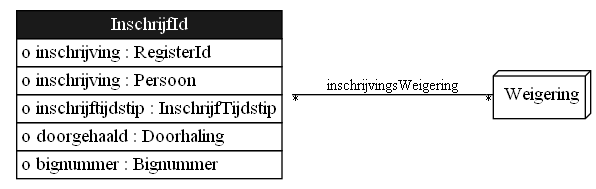
\includegraphics{C:/Users/gerar/OneDrive/OU/master/SE graduation/uitvoering/pattern/docs/images/RelationsInPatternWeigering.dot}
\caption{Figuur 3.1: Conceptueel diagram van relaties in
Weigering}\label{fig:Conceptueelux20diagramux20vanux20relatiesux20inux20Weigering}
}
\end{figure}

3.2
 geeft een conceptueel diagram met alle relaties die gedeclareerd zijn in ‘Aantekening’.

\begin{figure}
\hypertarget{fig:Conceptueelux20diagramux20vanux20relatiesux20inux20Aantekening}{%
\centering
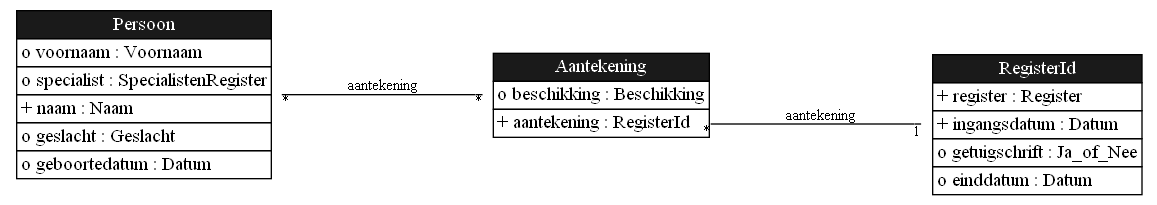
\includegraphics{C:/Users/gerar/OneDrive/OU/master/SE graduation/uitvoering/pattern/docs/images/RelationsInPatternAantekening.dot}
\caption{Figuur 3.2: Conceptueel diagram van relaties in
Aantekening}\label{fig:Conceptueelux20diagramux20vanux20relatiesux20inux20Aantekening}
}
\end{figure}

3.3
 geeft een conceptueel diagram met alle relaties die gedeclareerd zijn in ‘Specialisme’.

\begin{figure}
\hypertarget{fig:Conceptueelux20diagramux20vanux20relatiesux20inux20Specialisme}{%
\centering
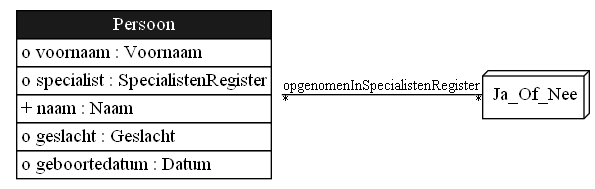
\includegraphics{C:/Users/gerar/OneDrive/OU/master/SE graduation/uitvoering/pattern/docs/images/RelationsInPatternSpecialisme.dot}
\caption{Figuur 3.3: Conceptueel diagram van relaties in
Specialisme}\label{fig:Conceptueelux20diagramux20vanux20relatiesux20inux20Specialisme}
}
\end{figure}

3.4
 geeft een conceptueel diagram met alle relaties die gedeclareerd zijn in ‘Inschrijfduur’.

\begin{figure}
\hypertarget{fig:Conceptueelux20diagramux20vanux20relatiesux20inux20Inschrijfduur}{%
\centering
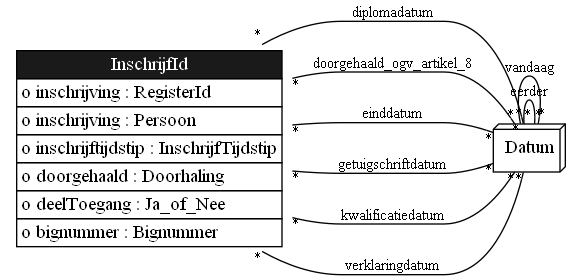
\includegraphics{C:/Users/gerar/OneDrive/OU/master/SE graduation/uitvoering/pattern/docs/images/RelationsInPatternInschrijfduur.dot}
\caption{Figuur 3.4: Conceptueel diagram van relaties in
Inschrijfduur}\label{fig:Conceptueelux20diagramux20vanux20relatiesux20inux20Inschrijfduur}
}
\end{figure}

3.5
 geeft een conceptueel diagram met alle relaties die gedeclareerd zijn in ‘Inschrijving’.

\begin{figure}
\hypertarget{fig:Conceptueelux20diagramux20vanux20relatiesux20inux20Inschrijving}{%
\centering
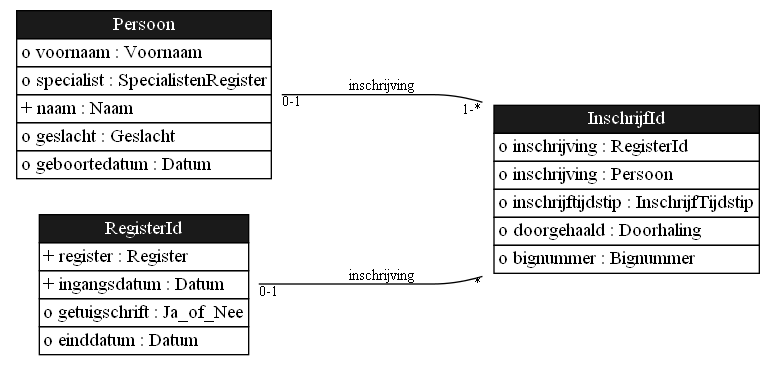
\includegraphics{C:/Users/gerar/OneDrive/OU/master/SE graduation/uitvoering/pattern/docs/images/RelationsInPatternInschrijving.dot}
\caption{Figuur 3.5: Conceptueel diagram van relaties in
Inschrijving}\label{fig:Conceptueelux20diagramux20vanux20relatiesux20inux20Inschrijving}
}
\end{figure}

3.6
 geeft een conceptueel diagram met alle relaties die gedeclareerd zijn in ‘Register’.

\begin{figure}
\hypertarget{fig:Conceptueelux20diagramux20vanux20relatiesux20inux20Register}{%
\centering
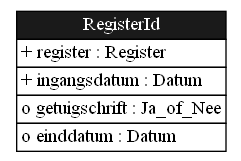
\includegraphics{C:/Users/gerar/OneDrive/OU/master/SE graduation/uitvoering/pattern/docs/images/RelationsInPatternRegister.dot}
\caption{Figuur 3.6: Conceptueel diagram van relaties in
Register}\label{fig:Conceptueelux20diagramux20vanux20relatiesux20inux20Register}
}
\end{figure}

3.7
 geeft een conceptueel diagram met alle relaties die gedeclareerd zijn in ‘Arts’.

\begin{figure}
\hypertarget{fig:Conceptueelux20diagramux20vanux20relatiesux20inux20Arts}{%
\centering
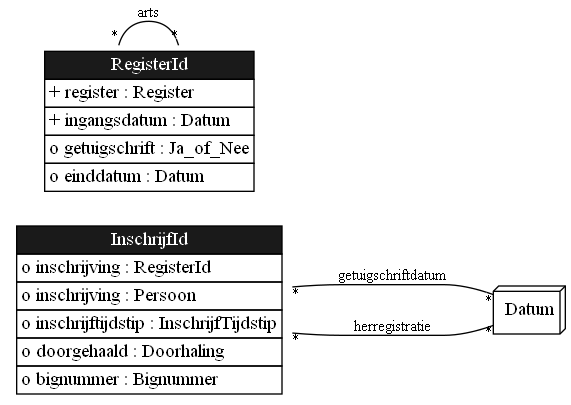
\includegraphics{C:/Users/gerar/OneDrive/OU/master/SE graduation/uitvoering/pattern/docs/images/RelationsInPatternArts.dot}
\caption{Figuur 3.7: Conceptueel diagram van relaties in
Arts}\label{fig:Conceptueelux20diagramux20vanux20relatiesux20inux20Arts}
}
\end{figure}

3.8
 geeft een conceptueel diagram met alle relaties die gedeclareerd zijn in ‘Tandarts’.

\begin{figure}
\hypertarget{fig:Conceptueelux20diagramux20vanux20relatiesux20inux20Tandarts}{%
\centering
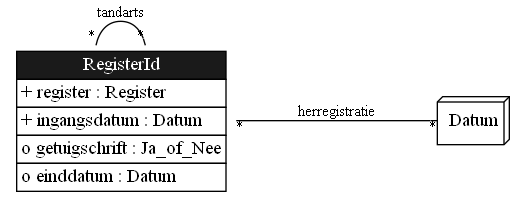
\includegraphics{C:/Users/gerar/OneDrive/OU/master/SE graduation/uitvoering/pattern/docs/images/RelationsInPatternTandarts.dot}
\caption{Figuur 3.8: Conceptueel diagram van relaties in
Tandarts}\label{fig:Conceptueelux20diagramux20vanux20relatiesux20inux20Tandarts}
}
\end{figure}

3.9
 geeft een conceptueel diagram met alle relaties die gedeclareerd zijn in ‘Apotheker’.

\begin{figure}
\hypertarget{fig:Conceptueelux20diagramux20vanux20relatiesux20inux20Apotheker}{%
\centering
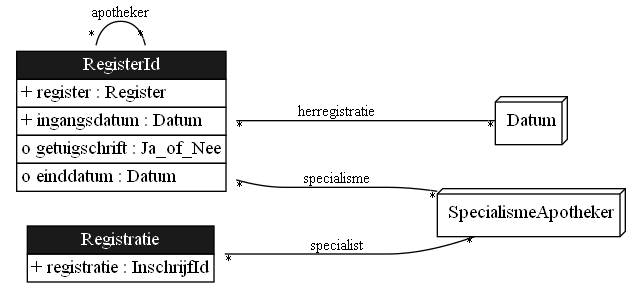
\includegraphics{C:/Users/gerar/OneDrive/OU/master/SE graduation/uitvoering/pattern/docs/images/RelationsInPatternApotheker.dot}
\caption{Figuur 3.9: Conceptueel diagram van relaties in
Apotheker}\label{fig:Conceptueelux20diagramux20vanux20relatiesux20inux20Apotheker}
}
\end{figure}

3.10
 geeft een conceptueel diagram met alle relaties die gedeclareerd zijn in ‘Geslacht’.

\begin{figure}
\hypertarget{fig:Conceptueelux20diagramux20vanux20relatiesux20inux20Geslacht}{%
\centering
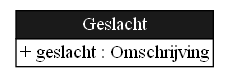
\includegraphics{C:/Users/gerar/OneDrive/OU/master/SE graduation/uitvoering/pattern/docs/images/RelationsInPatternGeslacht.dot}
\caption{Figuur 3.10: Conceptueel diagram van relaties in
Geslacht}\label{fig:Conceptueelux20diagramux20vanux20relatiesux20inux20Geslacht}
}
\end{figure}

3.11
 geeft een conceptueel diagram met alle relaties die gedeclareerd zijn in ‘Nationaliteit’.

\begin{figure}
\hypertarget{fig:Conceptueelux20diagramux20vanux20relatiesux20inux20Nationaliteit}{%
\centering
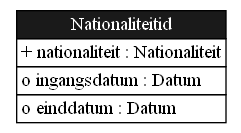
\includegraphics{C:/Users/gerar/OneDrive/OU/master/SE graduation/uitvoering/pattern/docs/images/RelationsInPatternNationaliteit.dot}
\caption{Figuur 3.11: Conceptueel diagram van relaties in
Nationaliteit}\label{fig:Conceptueelux20diagramux20vanux20relatiesux20inux20Nationaliteit}
}
\end{figure}

3.12
 geeft een conceptueel diagram met alle relaties die gedeclareerd zijn in ‘Adres’.

\begin{figure}
\hypertarget{fig:Conceptueelux20diagramux20vanux20relatiesux20inux20Adres}{%
\centering
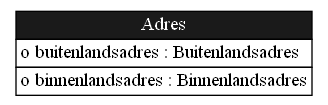
\includegraphics{C:/Users/gerar/OneDrive/OU/master/SE graduation/uitvoering/pattern/docs/images/RelationsInPatternAdres.dot}
\caption{Figuur 3.12: Conceptueel diagram van relaties in
Adres}\label{fig:Conceptueelux20diagramux20vanux20relatiesux20inux20Adres}
}
\end{figure}

De volgende regel heeft noch oogmerk (purpose), noch betekenis:

\begin{itemize}
\item
  \emph{Initialize today's date}
  (C:\textbackslash Users\textbackslash gerar\textbackslash OneDrive\textbackslash OU\textbackslash master\textbackslash SE graduation\textbackslash uitvoering\textbackslash pattern\textbackslash big\textbackslash generiek\textbackslash Generic.adl:23:5)

  \(I_{ \lbrack SESSION \rbrack }\vdash sessionToday;sessionToday^{\smallsmile}\)

  Voor alle s, s': Als s is equivalent met s' dan (Er is een d: s
  sessionToday d en s' sessionToday d)
\end{itemize}

Van de volgende regels is het oogmerk (purpose) niet uitgelegd:

\begin{itemize}
\item
  \emph{Elke nationaliteit heeft een ingangsdatum}
  (C:\textbackslash Users\textbackslash gerar\textbackslash OneDrive\textbackslash OU\textbackslash master\textbackslash SE graduation\textbackslash uitvoering\textbackslash pattern\textbackslash big\textbackslash generiek\textbackslash Nationaliteit.adl:47:9)

  \(I_{ \lbrack Nationaliteitid \rbrack }\vdash ingangsdatum;ingangsdatum^{\smallsmile}\)

  Voor alle n, n': Als n is equivalent met n' dan (Er is een d: De
  Nationaliteit n heeft als ingangsdatum d. en De Nationaliteit n' heeft
  als ingangsdatum d.)
\item
  \emph{Elke persoon heeft een nationaliteit}
  (C:\textbackslash Users\textbackslash gerar\textbackslash OneDrive\textbackslash OU\textbackslash master\textbackslash SE graduation\textbackslash uitvoering\textbackslash pattern\textbackslash big\textbackslash generiek\textbackslash Persoon.adl:104:9)

  \(I_{ \lbrack Persoon \rbrack }\vdash nationaliteit;nationaliteit^{\smallsmile}\)

  Voor alle p, p': Als p is equivalent met p' dan (Er is een n: p
  nationaliteit n en p' nationaliteit n)
\item
  \emph{TotAdres}
  (C:\textbackslash Users\textbackslash gerar\textbackslash OneDrive\textbackslash OU\textbackslash master\textbackslash SE graduation\textbackslash uitvoering\textbackslash pattern\textbackslash big\textbackslash generiek\textbackslash Persoon.adl:118:9)

  \(I_{ \lbrack Persoon \rbrack }\vdash adres;adres^{\smallsmile}\)

  Voor alle p, p': Als p is equivalent met p' dan (Er is een a: p adres
  a en p' adres a)
\item
  \emph{TotGeboortedatum}
  (C:\textbackslash Users\textbackslash gerar\textbackslash OneDrive\textbackslash OU\textbackslash master\textbackslash SE graduation\textbackslash uitvoering\textbackslash pattern\textbackslash big\textbackslash generiek\textbackslash Persoon.adl:78:9)

  \(I_{ \lbrack Persoon \rbrack }\vdash geboortedatum;geboortedatum^{\smallsmile}\)

  Voor alle p, p': Als p is equivalent met p' dan (Er is een d: p
  geboortedatum d en p' geboortedatum d)
\item
  \emph{TotGeslacht}
  (C:\textbackslash Users\textbackslash gerar\textbackslash OneDrive\textbackslash OU\textbackslash master\textbackslash SE graduation\textbackslash uitvoering\textbackslash pattern\textbackslash big\textbackslash generiek\textbackslash Persoon.adl:91:9)

  \(I_{ \lbrack Persoon \rbrack }\vdash geslacht;geslacht^{\smallsmile}\)

  Voor alle p, p': Als p is equivalent met p' dan (Er is een g: p
  geslacht g en p' geslacht g)
\item
  \emph{TotGetuigschrift}
  (C:\textbackslash Users\textbackslash gerar\textbackslash OneDrive\textbackslash OU\textbackslash master\textbackslash SE graduation\textbackslash uitvoering\textbackslash pattern\textbackslash big\textbackslash generiek\textbackslash Register.adl:76:9)

  \(I_{ \lbrack RegisterId \rbrack }\vdash getuigschrift;getuigschrift^{\smallsmile}\)

  Voor alle r, r': Als r is equivalent met r' dan (Er is een j: r
  getuigschrift j en r' getuigschrift j)
\item
  \emph{TotInschrijvingBig}
  (C:\textbackslash Users\textbackslash gerar\textbackslash OneDrive\textbackslash OU\textbackslash master\textbackslash SE graduation\textbackslash uitvoering\textbackslash pattern\textbackslash big\textbackslash generiek\textbackslash Inschrijving.adl:73:13)

  \(I_{ \lbrack InschrijfId \rbrack }\vdash bignummer;bignummer^{\smallsmile}\)

  Voor alle i, i': Als i is equivalent met i' dan (Er is een b: i
  bignummer b en i' bignummer b)
\item
  \emph{TotNaam}
  (C:\textbackslash Users\textbackslash gerar\textbackslash OneDrive\textbackslash OU\textbackslash master\textbackslash SE graduation\textbackslash uitvoering\textbackslash pattern\textbackslash big\textbackslash generiek\textbackslash Persoon.adl:50:9)

  \(I_{ \lbrack Persoon \rbrack }\vdash naam;naam^{\smallsmile}\)

  Voor alle p, p': Als p is equivalent met p' dan (Er is een n: De
  persoon met het id p wordt n genoemd. en De persoon met het id p'
  wordt n genoemd.)
\item
  \emph{TotVoornaam}
  (C:\textbackslash Users\textbackslash gerar\textbackslash OneDrive\textbackslash OU\textbackslash master\textbackslash SE graduation\textbackslash uitvoering\textbackslash pattern\textbackslash big\textbackslash generiek\textbackslash Persoon.adl:64:9)

  \(I_{ \lbrack Persoon \rbrack }\vdash voornaam;voornaam^{\smallsmile}\)

  Voor alle p, p': Als p is equivalent met p' dan (Er is een v: De
  persoon met het id p heeft v als voornaam. en De persoon met het id p'
  heeft v als voornaam.)
\end{itemize}

De volgende regels gaan niet vergezeld van een betekenis in natuurlijke taal:

\begin{itemize}
\item
  \emph{Create Inschrijving}
  (C:\textbackslash Users\textbackslash gerar\textbackslash OneDrive\textbackslash OU\textbackslash master\textbackslash SE graduation\textbackslash uitvoering\textbackslash pattern\textbackslash big\textbackslash generiek\textbackslash Persoon.adl:126:9)

  \(I_{ \lbrack Persoon \rbrack }\vdash inschrijving;inschrijving^{\smallsmile}\)

  Voor alle p, p': Als p is equivalent met p' dan (Er is een i: p
  inschrijving i en p' inschrijving i)
\item
  \emph{Voeg datum registratie toe}
  (C:\textbackslash Users\textbackslash gerar\textbackslash OneDrive\textbackslash OU\textbackslash master\textbackslash SE graduation\textbackslash uitvoering\textbackslash pattern\textbackslash big\textbackslash generiek\textbackslash Registratie.adl:52:13)

  \(I_{ \lbrack Registratie \rbrack }\vdash registratiedatum;registratiedatum^{\smallsmile}\)

  Voor alle r, r': Als r is equivalent met r' dan (Er is een d: r
  registratiedatum d en r' registratiedatum d)
\item
  \emph{Voeg\_Bignummer\_toe(automatisch)}
  (C:\textbackslash Users\textbackslash gerar\textbackslash OneDrive\textbackslash OU\textbackslash master\textbackslash SE graduation\textbackslash uitvoering\textbackslash pattern\textbackslash big\textbackslash generiek\textbackslash Inschrijving.adl:83:13)

  \(I_{ \lbrack InschrijfId \rbrack }\vdash bignummer;bignummer^{\smallsmile}\)

  Voor alle i, i': Als i is equivalent met i' dan (Er is een b: i
  bignummer b en i' bignummer b)
\item
  \emph{Voeg\_Registratie\_toe(automatisch)}
  (C:\textbackslash Users\textbackslash gerar\textbackslash OneDrive\textbackslash OU\textbackslash master\textbackslash SE graduation\textbackslash uitvoering\textbackslash pattern\textbackslash big\textbackslash generiek\textbackslash Registratie.adl:42:13)

  \(I_{ \lbrack InschrijfId \rbrack }\cap inschrijving^{\smallsmile};inschrijving\vdash registratie^{\smallsmile};registratie\)

  Voor alle i, i': Als (i is equivalent met i') en (Er is een r': r'
  inschrijving i en r' inschrijving i') dan (Er is een r': r'
  registratie i en r' registratie i')
\item
  \emph{Voeg\_inschrijftijd\_toe\_(automatisch)}
  (C:\textbackslash Users\textbackslash gerar\textbackslash OneDrive\textbackslash OU\textbackslash master\textbackslash SE graduation\textbackslash uitvoering\textbackslash pattern\textbackslash big\textbackslash generiek\textbackslash Inschrijving.adl:48:13)

  \(I_{ \lbrack InschrijfId \rbrack }\vdash inschrijftijdstip;inschrijftijdstip^{\smallsmile}\)

  Voor alle i, i': Als i is equivalent met i' dan (Er is een i'': i
  inschrijftijdstip i'' en i' inschrijftijdstip i'')
\end{itemize}

Onderstaande tabel bevat per thema (dwz. patroon) tellingen van het aantal relaties en regels, gevolgd door het aantal en het percentage daarvan dat een referentie bevat. Relaties die in meerdere thema's gedeclareerd worden, worden ook meerdere keren geteld.

\begin{longtable}[]{@{}
  >{\raggedright\arraybackslash}p{(\columnwidth - 12\tabcolsep) * \real{0.40}}
  >{\centering\arraybackslash}p{(\columnwidth - 12\tabcolsep) * \real{0.10}}
  >{\centering\arraybackslash}p{(\columnwidth - 12\tabcolsep) * \real{0.10}}
  >{\centering\arraybackslash}p{(\columnwidth - 12\tabcolsep) * \real{0.10}}
  >{\centering\arraybackslash}p{(\columnwidth - 12\tabcolsep) * \real{0.10}}
  >{\centering\arraybackslash}p{(\columnwidth - 12\tabcolsep) * \real{0.10}}
  >{\centering\arraybackslash}p{(\columnwidth - 12\tabcolsep) * \real{0.10}}@{}}
\toprule
Thema & & & & & & \\
Relaties & & & & & & \\
Met referentie & & & & & & \\
\% & & & & & & \\
Regels & & & & & & \\
Gehele context & & & & & & \\
\% & & & & & & \\
\midrule
\endhead
Weigering & 1 & 0 & 0\% & 0 & 0 & - \\
Aantekening & 3 & 0 & 0\% & 0 & 0 & - \\
Specialisme & 2 & 0 & 0\% & 0 & 0 & - \\
Inschrijfduur & 8 & 0 & 0\% & 0 & 0 & - \\
Registratie & 2 & 0 & 0\% & 2 & 0 & 0\% \\
Inschrijving & 4 & 0 & 0\% & 3 & 0 & 0\% \\
Register & 4 & 0 & 0\% & 1 & 0 & 0\% \\
Arts & 3 & 0 & 0\% & 0 & 0 & - \\
Tandarts & 3 & 0 & 0\% & 0 & 0 & - \\
Apotheker & 3 & 0 & 0\% & 0 & 0 & - \\
Geslacht & 1 & 0 & 0\% & 0 & 0 & - \\
Nationaliteit & 3 & 0 & 0\% & 1 & 0 & 0\% \\
Adres & 2 & 0 & 0\% & 0 & 0 & - \\
Persoon & 6 & 0 & 0\% & 7 & 0 & 0\% \\
Gehele context & 45 & 0 & 0\% & 15 & 0 & 0\% \\
\bottomrule
\end{longtable}

Onderstaande tabel bevat een overzicht van de signaalregels per rol.

\begin{longtable}[]{@{}
  >{\raggedright\arraybackslash}p{(\columnwidth - 4\tabcolsep) * \real{0.33}}
  >{\raggedright\arraybackslash}p{(\columnwidth - 4\tabcolsep) * \real{0.33}}
  >{\raggedright\arraybackslash}p{(\columnwidth - 4\tabcolsep) * \real{0.33}}@{}}
\toprule
rol & & \\
thema & & \\
regel & & \\
\midrule
\endhead
ExecEngine & Inschrijfduur &
Compute kwalificatiedatum{[}InschrijfId*Datum{]} using DelPair \\
ExecEngine & Inschrijfduur &
Compute kwalificatiedatum{[}InschrijfId*Datum{]} using InsPair \\
ExecEngine & Persoon & Create Inschrijving \\
USER & Nationaliteit & Elke nationaliteit heeft een ingangsdatum \\
USER & Persoon & Elke persoon heeft een nationaliteit \\
ExecEngine & -\/- & Initialize today's date \\
USER & Persoon & TotAdres \\
USER & Persoon & TotGeboortedatum \\
USER & Persoon & TotGeslacht \\
USER & Register & TotGetuigschrift \\
USER & Inschrijving & TotInschrijvingBig \\
USER & Persoon & TotNaam \\
USER & Persoon & TotVoornaam \\
ExecEngine & Registratie & Voeg datum registratie toe \\
ExecEngine & Inschrijving & Voeg\_Bignummer\_toe(automatisch) \\
ExecEngine & Registratie & Voeg\_Registratie\_toe(automatisch) \\
ExecEngine & Inschrijving & Voeg\_inschrijftijd\_toe\_(automatisch) \\
\bottomrule
\end{longtable}

Dit script bevat onderhanden werk. De volgende tabellen geven details met regelnummers in de oorspronkelijk script-bestanden.

\begin{longtable}[]{@{}
  >{\raggedright\arraybackslash}p{(\columnwidth - 4\tabcolsep) * \real{0.33}}
  >{\raggedleft\arraybackslash}p{(\columnwidth - 4\tabcolsep) * \real{0.33}}
  >{\raggedleft\arraybackslash}p{(\columnwidth - 4\tabcolsep) * \real{0.33}}@{}}
\toprule
regel & & \\
locatie & & \\
\#taken & & \\
\midrule
\endhead
Voeg datum registratie toe &
C:\textbackslash Users\textbackslash gerar\textbackslash OneDrive\textbackslash OU\textbackslash master\textbackslash SE graduation\textbackslash uitvoering\textbackslash pattern\textbackslash big\textbackslash generiek\textbackslash Registratie.adl:52:13
& 1 \\
Voeg\_Registratie\_toe(automatisch) &
C:\textbackslash Users\textbackslash gerar\textbackslash OneDrive\textbackslash OU\textbackslash master\textbackslash SE graduation\textbackslash uitvoering\textbackslash pattern\textbackslash big\textbackslash generiek\textbackslash Registratie.adl:42:13
& 2 \\
Voeg\_inschrijftijd\_toe\_(automatisch) &
C:\textbackslash Users\textbackslash gerar\textbackslash OneDrive\textbackslash OU\textbackslash master\textbackslash SE graduation\textbackslash uitvoering\textbackslash pattern\textbackslash big\textbackslash generiek\textbackslash Inschrijving.adl:48:13
& 3 \\
\bottomrule
\end{longtable}

Afspraak {[} @agr:SharedLangrule-\/-1483780593 {]} (
‘Voeg datum registratie toe’ ) luidt: 

Deze regel bevat nog werk (voor ExecEngine), te weten ‘RegistratieR001’.

Afspraak {[} @agr:SharedLangrule-119394377 {]} (
‘Voeg\_Registratie\_toe(automatisch)’ ) luidt: 

Deze regel bevat nog werk (voor ExecEngine). De volgende tabel laat de items zien die aandacht vragen.

\begin{longtable}[]{@{}
  >{\raggedright\arraybackslash}p{(\columnwidth - 2\tabcolsep) * \real{0.50}}
  >{\raggedright\arraybackslash}p{(\columnwidth - 2\tabcolsep) * \real{0.50}}@{}}
\toprule
InschrijfId & \\
InschrijfId & \\
\midrule
\endhead
I003 & I003 \\
I002 & I002 \\
\bottomrule
\end{longtable}

Afspraak {[} @agr:SharedLangrule-\/-1033180058 {]} (
‘Voeg\_inschrijftijd\_toe\_(automatisch)’ ) luidt: 

Deze regel bevat nog werk (voor ExecEngine). De volgende tabel laat de items zien die aandacht vragen.

\begin{longtable}[]{@{}
  >{\raggedright\arraybackslash}p{(\columnwidth - 0\tabcolsep) * \real{1.00}}@{}}
\toprule
InschrijfId \\
\midrule
\endhead
I001 \\
I003 \\
I002 \\
\bottomrule
\end{longtable}

De populatie in dit script overtreedt 0 invarianten en 3 procesregels.

\begin{itemize}
\item
  \emph{Regel Voeg datum registratie toe}

  Totaal aantal taken: 1

  \begin{longtable}[]{@{}
    >{\raggedright\arraybackslash}p{(\columnwidth - 0\tabcolsep) * \real{1.00}}@{}}
  \toprule
  \endhead
  \textbf{There is one violation of RULE "Voeg datum registratie toe":
  \{EX\}
  InsPair;registratiedatum;Registratie;"R001";Datum;\{php\}date(DATE\_ISO8601)
  } \\
  \bottomrule
  \end{longtable}
\item
  \emph{Regel Voeg\_Registratie\_toe(automatisch)}

  Totaal aantal taken: 2

  \begin{longtable}[]{@{}
    >{\raggedright\arraybackslash}p{(\columnwidth - 0\tabcolsep) * \real{1.00}}@{}}
  \toprule
  \endhead
  \textbf{There are 2 violations of RULE
  "Voeg\_Registratie\_toe(automatisch)": \{EX\}
  InsAtom;Registratie\{EX\}
  InsPair;registratie;Registratie;\_NEW;InschrijfId;"I003" \{EX\}
  InsAtom;Registratie\{EX\}
  InsPair;registratie;Registratie;\_NEW;InschrijfId;"I002" } \\
  \bottomrule
  \end{longtable}
\item
  \emph{Regel Voeg\_inschrijftijd\_toe\_(automatisch)}

  Totaal aantal taken: 3

  \begin{longtable}[]{@{}
    >{\raggedright\arraybackslash}p{(\columnwidth - 0\tabcolsep) * \real{1.00}}@{}}
  \toprule
  \endhead
  \textbf{There are 3 violations of RULE
  "Voeg\_inschrijftijd\_toe\_(automatisch)": \{EX\}
  InsAtom;InschrijfTijdstip\{EX\}
  InsPair;inschrijftijdstip;InschrijfId;"I001";InschrijfTijdstip;\{php\}date(DATE\_ISO8601)
  \{EX\} InsAtom;InschrijfTijdstip\{EX\}
  InsPair;inschrijftijdstip;InschrijfId;"I003";InschrijfTijdstip;\{php\}date(DATE\_ISO8601)
  \{EX\} InsAtom;InschrijfTijdstip\{EX\}
  InsPair;inschrijftijdstip;InschrijfId;"I002";InschrijfTijdstip;\{php\}date(DATE\_ISO8601)
  } \\
  \bottomrule
  \end{longtable}
\end{itemize}

\hypertarget{sec:ConceptualAnalysis}{%
\chapter{Conceptuele Analyse}\label{sec:ConceptualAnalysis}}

Dit hoofdstuk analyseert de "taal van de business", om functionele eisen
ten behoeve van ‘Big’ te kunnen bespreken. Deze analyse beoogt om een
bouwbare, maar oplossingsonafhankelijke specificatie op te leveren. Het
begrijpen van tekst vereist deskundigheid op het gebied van conceptueel
modelleren.

\section{De wet BIG}

Het BIG-register is onderdeel van de Wet op de beroepen in de
individuele gezondheidszorg (BIG). Het doel van de Wet BIG is te zorgen
dat de kwaliteit van onze gezondheidszorg hoog is en blijft. Ook
beschermt de Wet BIG patiënten tegen ondeskundig en onzorgvuldig
handelen van zorgverleners.

De Wet BIG verdeelt beroepen die onder deze wet vallen in 3 groepen
volgens hun wettelijke artikelnummer: artikel 3-, 34- en artikel
36a-beroepen. In het BIG-register worden alleen artikel 3 en artikel
36a-beroepen geregistreerd. Daarnaast bestaan er ook wettelijk erkende
specialismen. Deze vallen onder artikel 14. Een specialisme wordt
aangetekend bij een artikel 3 beroep. Beroepen die in het BIG-register
staan geregistreerd vallen onder het tuchtrecht.

Naast het registreren en herregistreren van deze beroepsbeoefenaren en
de uitvoering van het tuchtrecht valt ook het erkennen van
(buitenlandse) diploma’s en onder de taken van het BIG-register.
Zorgverleners met een buitenlands diploma moeten voldoen aan de
Nederlandse opleidingseisen. Hun opleidingsniveau moet gelijk zijn aan
dat van een zorgverlener met een Nederlands diploma. Eventueel telt
relevante werkervaring mee om het niveau te bepalen. Het CIBG neemt
hierover een besluit op grond van het advies van de onafhankelijke
deskundigencommissie, de Commissie buitenslands gediplomeerden
volksgezondheid (CBGV).

Tevens kunnen zorgprofessionals bij het BIG-register terecht voor het
aanvragen van verklaringen en zorgt het bigregister voor het aantekenen
van specialismen en voorschrijfbevoegdheden.

Voor zorgconsumenten en organisaties biedt het BIG-register de
mogelijkheid te controleren of zijn zorgverlener bevoegd is om zijn of
haar beroep uit te oefenen.

\subsection{Opdrachtgever}

De Directie MEVA van het Ministerie van VWS is opdrachtgever voor de
uitvoering van de Wet BIG.

\subsection{Onderliggende wetgeving}

\begin{itemize}
\tightlist
\item
  \href{https://wetten.overheid.nl/BWBR0006251/2021-07-01}{Wet op de
  beroepen in de individuele gezondheidszorg}
\item
  \href{https://wetten.overheid.nl/BWBR0024841/2020-07-01}{Besluit
  periodieke registratie Wet BIG}
\item
  \href{https://wetten.overheid.nl/BWBR0007648/2021-01-01}{Registratiebesluit
  BIG}
\item
  \href{https://wetten.overheid.nl/BWBR0008688/2021-04-01}{Tuchtrechtbesluit
  BIG}
\item
  \href{https://wetten.overheid.nl/BWBR0025605/2020-12-15}{Regeling
  periodieke registratie Wet BIG}
\item
  \href{https://wetten.overheid.nl/BWBR0031720/2014-02-01}{Regeling
  tarieven registratie beroepsbeoefenaren Wet BIG}
\end{itemize}

Het BIGregister bevindt zich in een keten van informatieverstrekking en
is sterk afhankelijk van informatie van derden. Zo zijn derden weer
sterk afhankelijk van onze informatie.

\subsection{Huidig informatiesysteem}

De Wet BIG stamt uit 1993. Het huidige zaaksysteem (Zorro) is als
opvolger van Ribiz ontwikkeld in 2007. Eind 2018 is het eerste deel van
de publieke website vernieuwd. Medio 2019 volgt vernieuwing van een
volgend deel van de publieke website, waarmee op dat moment alleen de
advieswijzer nog niet is omgezet.

\hypertarget{sec:SharedLangtheme-525340773}{%
\section{Weigering}\label{sec:SharedLangtheme-525340773}}

De inschrijving wordt geweigerd:

\begin{enumerate}
\tightlist
\item
  indien de aanvrager niet voldoet aan de in hoofdstuk III bedoelde
  opleidingseisen;
\item
  indien de aanvrager ingevolge in kracht van gewijsde gegane
  rechterlijke uitspraak onder curatele is gesteld wegens lichamelijke
  of geestelijke toestand;
\item
  indien de aanvrager ingevolge rechterlijke uitspraak ontzet is van het
  recht het betrokken beroep uit te oefenen;
\item
  indien zulks voortvloeit uit een op grond van deze wet jegens de
  aanvrager genomen maatregel;
\item
  indien ten aanzien van de aanvrager een maatregel, berustende op een
  in het buitenland gegeven rechterlijke, tuchtrechtelijke of
  bestuursrechtelijke beslissing, van kracht is op grond waarvan de
  aanvrager zijn rechten ter zake van de uitoefening van het betrokken
  beroep in het land waar de beslissing is gegeven tijdelijk of blijvend
  geheel heeft verloren,
\item
  indien de aanvrager de Nederlandse taal niet voldoende beheerst om
  zijn beroep in Nederland uit te kunnen oefenen.
\end{enumerate}

\begin{description}
\tightlist
\item[Definitie 0:]
art.6-redenen voor afwijzing inschrijving.
\end{description}

4.1 Conceptueel diagram van ‘Weigering’.

\begin{figure}
\hypertarget{fig:Conceptueelux20diagramux20vanux20Weigering}{%
\centering
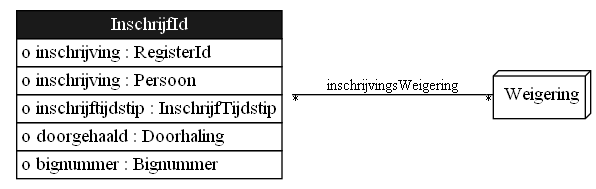
\includegraphics{C:/Users/gerar/OneDrive/OU/master/SE graduation/uitvoering/pattern/docs/images/CDPatternWeigering.dot}
\caption{Figuur 4.1: Conceptueel diagram van
Weigering}\label{fig:Conceptueelux20diagramux20vanux20Weigering}
}
\end{figure}

\begin{longtable}[]{@{}ll@{}}
\toprule
Relatie & Betekenis \\
\midrule
\endhead
inschrijvingsWeigering {[}InschrijfId*Weigering{]} & In artikel 6 staan
de redenen voor het weigeren van de inschrijving bepaald. \\
\bottomrule
\end{longtable}

\hypertarget{sec:SharedLangtheme-958700505}{%
\section{Aantekening}\label{sec:SharedLangtheme-958700505}}

Artikel 9 1. In het register wordt, indien zulks voortvloeit uit een op
grond van deze wet genomen maatregel of besluit, een aantekening
geplaatst van: a. een opgelegde berisping indien dit op grond van
artikel 48, elfde lid, door het regionale tuchtcollege of het centraal
tuchtcollege is beslist; b. een opgelegde geldboete indien dit op grond
van artikel 48, elfde lid, door het regionale tuchtcollege of het
centraal tuchtcollege is beslist; c. de schorsing van de bevoegdheid,
bedoeld in artikel 48, eerste lid, onder d; d. de voorwaarden die zijn
opgelegd; e. de gedeeltelijke ontzegging van de bevoegdheid het
betrokken beroep uit te oefenen; f. de doorhaling van de inschrijving in
het register op grond van artikel 7, onder c, d of e; g. de ontzegging
van het recht wederom in het register te worden ingeschreven; h. het
eindigen van een schorsing, anders dan ten gevolge van het verstrijken
van de in een maatregel vastgestelde tijdsduur; i. het niet langer
gelden van de onder e bedoelde voorwaarden, anders dan ten gevolge van
het verstrijken van de proeftijd, en van de onder f bedoelde ontzegging;
j. de bevoegdheid van een krachtens artikel 5 aangewezen
beroepsbeoefenaar om de krachtens artikel 36, veertiende lid, aangewezen
UR-geneesmiddelen voor te schrijven, onder vermelding van de categorie
van beroepsbeoefenaren waartoe de betrokken beroepsbeoefenaar behoort;
k. de op grond van artikel 48, tweede lid, opgelegde beperkingen met
betrekking tot het beroepsmatig handelen op het gebied van de
individuele gezondheidszorg; l. de beslissing als bedoeld in artikel
48a, tweede lid, tot de tenuitvoerlegging van een voorwaardelijke
maatregel; m. de last tot onmiddellijke onthouding van de
beroepsactiviteiten, bedoeld in artikel 85a. 2. In het register wordt
ten aanzien van een geregistreerd of voormalig geregistreerd
beroepsbeoefenaar een aantekening geplaatst van: a. een in het
buitenland gegeven rechterlijke, tuchtrechtelijke of bestuursrechtelijke
beslissing op grond waarvan de beroepsbeoefenaar zijn rechten ter zake
van de uitoefening van het recht het betrokken beroep uit te oefenen in
het land waar de beslissing is gegeven tijdelijk of blijvend geheel of
gedeeltelijk heeft verloren. Indien die rechterlijke uitspraak tevens
inhoudt een beperking in het recht om andere beroepen in de individuele
gezondheidszorg uit te oefenen, wordt die beperking eveneens
aangetekend. b. een op grond van de Wet medisch tuchtrecht BES gegeven
tuchtrechtelijke beslissing op grond waarvan de beroepsbeoefenaar zijn
rechten ter zake van de uitoefening van het betrokken beroep op Bonaire,
St. Eustatius en Saba tijdelijk of blijvend geheel of gedeeltelijk dan
wel voorwaardelijk heeft verloren. Indien die tuchtrechtelijk beslissing
tevens inhoudt een beperking in het recht om andere beroepen in de
individuele gezondheidszorg uit te oefenen, wordt die beperking eveneens
aangetekend. 3. In het register wordt een aantekening geplaatst van een
aan de beroepsbeoefenaar op grond van de Wet kwaliteit, klachten en
geschillen zorg gegeven bevel of aanwijzing, indien dat bevel of die
aanwijzing inhoudt dat aan de betrokkene een beperking is opgelegd in de
uitoefening van het betrokken beroep. 4. In het register wordt ten
aanzien van een geregistreerd of voormalig geregistreerd
beroepsbeoefenaar een aantekening geplaatst van: a. rechterlijke
uitspraken inhoudende de ontzetting van of beperking op het recht het
betrokken beroep uit te oefenen. Indien die rechterlijke uitspraak
tevens inhoudt een ontzetting van of beperking in het recht om ook
andere beroepen in de individuele gezondheidszorg uit te oefenen, wordt
die ontzetting of beperking eveneens aangetekend. b. een op grond van
artikel 14c, tweede lid, van het Wetboek van Strafrecht gestelde
bijzondere voorwaarde waaruit een inperking voortvloeit van de
bevoegdheid het betrokken beroep uit te oefenen. Indien die bijzondere
voorwaarde tevens inhoudt een beperking van de bevoegdheid om andere
beroepen in de individuele gezondheidszorg uit te oefenen, wordt die
inperking eveneens aangetekend. 5. Bij een aantekening als bedoeld in
het eerste tot en met vierde lid wordt vermeld: a. de datum waarop van
de schorsing een aantekening wordt geplaatst alsmede de duur van de
schorsing, indien die reeds bekend is; b. de datum waarop de berisping,
de geldboete, de in het eerste lid bedoelde voorwaarden, de ontzegging,
de doorhaling, de ontzegging van het recht op wederinschrijving, de last
tot onmiddellijke onthouding van de beroepsactiviteiten of het bevel of
de aanwijzing, bedoeld in het derde lid, zijn gaan gelden alsmede,
ingeval de voorwaarden of de in het tweede lid bedoelde maatregel tot
een proeftijd zijn beperkt, de duur daarvan dan wel c. de datum waarop
de schorsing of de last tot onmiddellijke onthouding van de
beroepsactiviteiten is geëindigd of vanaf welke de in eerste lid
bedoelde voorwaarden of de in het tweede en derde lid bedoelde
maatregelen niet langer gelden. 6. Indien de in het tweede lid bedoelde
aantekening in het register is geplaatst, geldt de in het buitenland dan
wel de op grond van de Wet medisch tuchtrecht BES opgelegde
bevoegdheidsbeperking ook voor de beroepsuitoefening in Nederland. 7. De
in het eerste, tweede, derde, vierde en achtste lid bedoelde aantekening
wordt gedurende een bij algemene maatregel van bestuur bepaalde termijn
in het register vermeld en daarbij wordt indien bekend de aard van het
vergrijp vermeld dat tot de aantekening heeft geleid, alsmede een met
redenen omklede toelichting op een genomen maatregel als bedoeld in
artikel 48, eerste lid, onder b en c. 8. In het register wordt voorts
een aantekening geplaatst van een maatregel als bedoeld in artikel 7,
eerste lid, onderdelen b en c, van de Wet medisch tuchtrecht BES, indien
dit op grond van artikel 7, vijfde lid, van de Wet medisch tuchtrecht
BES, door het College is beslist.

De aantekening wordt op het register geplaatst bij een
beroepsbeoefenaar. De aantekening heeft conform Artikel 9 betrekking op
het mogen uitvoeren van de zorgtaak.

\begin{description}
\tightlist
\item[Definitie 1:]
art.7a.2-zie artikel 9
\end{description}

4.2 Conceptueel diagram van ‘Aantekening’.

\begin{figure}
\hypertarget{fig:Conceptueelux20diagramux20vanux20Aantekening}{%
\centering
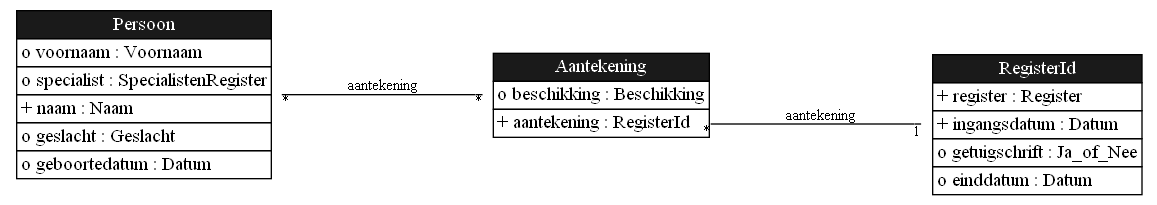
\includegraphics{C:/Users/gerar/OneDrive/OU/master/SE graduation/uitvoering/pattern/docs/images/CDPatternAantekening.dot}
\caption{Figuur 4.2: Conceptueel diagram van
Aantekening}\label{fig:Conceptueelux20diagramux20vanux20Aantekening}
}
\end{figure}

\begin{longtable}[]{@{}ll@{}}
\toprule
Relatie & Betekenis \\
\midrule
\endhead
aantekening {[}Aantekening*RegisterId{]} & Een aantekening als bedoeld
in artikel 9, tweede lid, onderdeel a van de Wet BIG is bedoeld om een
maatregel ten aanzien van een ingeschrevene te registreren. \\
aantekening {[}Persoon*Aantekening{]} & Bevat aantekening op een
Big-ingeschrevene. \\
beschikking {[}Aantekening*Beschikking{]} & Een register registreert een
beschikking als bedoeld in artikel 10 van de Wet BIG om een aantekening
in datzelfde register te onderbouwen. \\
\bottomrule
\end{longtable}

\hypertarget{sec:SharedLangtheme-492427277}{%
\section{Specialisme}\label{sec:SharedLangtheme-492427277}}

Een regeling als bedoeld in artikel 14, tweede lid, onder d, kan mede
inhouden dat degene die de opleiding tot specialist heeft voltooid wordt
ingeschreven als specialist voor een bij de regeling bepaalde periode en
dat een aansluitende hernieuwde inschrijving slechts plaatsvindt indien
de specialist gedurende een bij die regeling bepaald tijdvak,
voorafgaand aan de indiening van de aanvraag tot hernieuwde
inschrijving, regelmatig op het desbetreffende deelgebied van de
beroepsuitoefening werkzaam is geweest dan wel het beroep zal uitoefenen
onder de bij de hernieuwde inschrijving aan te geven
scholingsvoorwaarden.

\begin{description}
\tightlist
\item[Definitie 2:]
In artikel 8 lid 3 wordt aangegeven dat een ingeschrevene opgenomen in
kan zijn in een specialistenregister.
\end{description}

4.3 Conceptueel diagram van ‘Specialisme’.

\begin{figure}
\hypertarget{fig:Conceptueelux20diagramux20vanux20Specialisme}{%
\centering
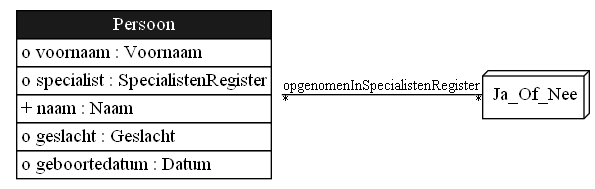
\includegraphics{C:/Users/gerar/OneDrive/OU/master/SE graduation/uitvoering/pattern/docs/images/CDPatternSpecialisme.dot}
\caption{Figuur 4.3: Conceptueel diagram van
Specialisme}\label{fig:Conceptueelux20diagramux20vanux20Specialisme}
}
\end{figure}

\begin{longtable}[]{@{}ll@{}}
\toprule
Relatie & Betekenis \\
\midrule
\endhead
opgenomenInSpecialistenRegister {[}Persoon*JaOfNee{]} & Zoals artikel 14
aangeeft kan een persoon opgenomen zijn in een specialistenregister. \\
specialist (Attribuut van Persoon) & Een Persoon is specialist wanneer
deze in het specialistenRegister is opgenomen. \\
\bottomrule
\end{longtable}

\hypertarget{sec:SharedLangtheme--1889304666}{%
\section{Inschrijfduur}\label{sec:SharedLangtheme--1889304666}}

Inschrijvingen in een register zijn beperkt geldig. Artikel 8, eerste
lid van de Wet BIG stelt: "Bij algemene maatregel van bestuur wordt
bepaald dat de inschrijving in een bij de maatregel aangewezen register
wordt doorgehaald indien na de in het tweede lid bedoelde datum een bij
de maatregel aangegeven periode is verstreken." Artikel 2, tweede lid
van het Besluit periodieke registratie Wet BIG stelt deze periode op
vijf jaren.

4.4 Conceptueel diagram van ‘Inschrijfduur’.

\begin{figure}
\hypertarget{fig:Conceptueelux20diagramux20vanux20Inschrijfduur}{%
\centering
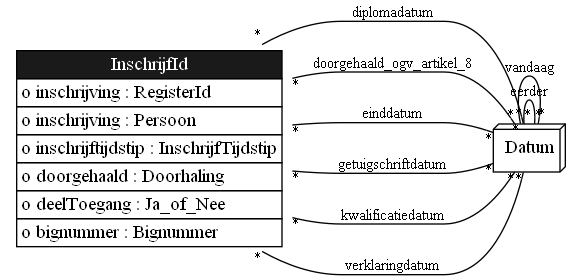
\includegraphics{C:/Users/gerar/OneDrive/OU/master/SE graduation/uitvoering/pattern/docs/images/CDPatternInschrijfduur.dot}
\caption{Figuur 4.4: Conceptueel diagram van
Inschrijfduur}\label{fig:Conceptueelux20diagramux20vanux20Inschrijfduur}
}
\end{figure}

\begin{longtable}[]{@{}
  >{\raggedright\arraybackslash}p{(\columnwidth - 2\tabcolsep) * \real{0.50}}
  >{\raggedright\arraybackslash}p{(\columnwidth - 2\tabcolsep) * \real{0.50}}@{}}
\toprule
Relatie & Betekenis \\
\midrule
\endhead
diplomadatum {[}InschrijfId*Datum{]} & Er is een erkend diploma bij een
inschrijving geregistreerd dat relevant is voor het bepalen van de
geldigheid van die inschrijving.

Een register registreert de datum waarop de ingeschrevene een diploma
heeft behaald op grond waarvan de ingeschrevene een erkenning van
beroepskwalificaties als bedoeld in de Algemene wet erkenning
EU-beroepskwalificaties heeft verkregen, zoals bedoeld in Art. 8 lid 2
sub a van de Wet BIG. Als er meerdere diploma's zijn, kunnen er dus ook
meerdere diplomadata zijn voor dezelfde inschrijving. \\
doorgehaald\_ogv\_artikel\_8 {[}InschrijfId*Datum{]} & Om het einde van
een inschrijving te bepalen tellen we vijf jaar (zie Artikel 2.2 van het
besluit) op bij de meest recente kwalificatiedatum. Als gevolg daarvan
verandert de einddatum als de ingeschrevene tijdig verlenging krijgt. \\
eerder {[}Datum*Datum{]} & Voor elke denkbare datum d1 en d2 geldt d1
eerder d2 dan en slechts dan als d1 \textless{} d2. \\
einddatum {[}InschrijfId*Datum{]} & Om het einde van een inschrijving te
bepalen tellen we vijf jaar (zie Artikel 2.2 van het besluit) op bij de
meest recente kwalificatiedatum. Als gevolg daarvan verandert de
einddatum als de ingeschrevene tijdig verlenging krijgt. \\
getuigschriftdatum {[}InschrijfId*Datum{]} & Er is een getuigschrift bij
een inschrijving geregistreerd dat relevant is voor het bepalen van de
geldigheid van die inschrijving.

Een register registreert datum waarop de ingeschrevene een bij of
krachtens hoofdstuk III of VI aangewezen getuigschrift heeft verkregen,
zoals bedoeld in Art. 8 lid 2 sub a van de Wet BIG. Als er meerdere
getuigschriften zijn, kunnen er dus ook meerdere data zijn bij dezelfde
inschrijving.

Een register registreert datum waarop de ingeschrevene een bij of
krachtens hoofdstuk III of VI aangewezen getuigschrift heeft verkregen,
zoals bedoeld in Art. 8 lid 2 sub a van de Wet BIG. Als er meerdere
getuigschriften zijn, kunnen er dus ook meerdere data zijn bij dezelfde
inschrijving.

Een register registreert datum waarop de ingeschrevene een bij of
krachtens hoofdstuk III of VI aangewezen getuigschrift heeft verkregen,
zoals bedoeld in Art. 8 lid 2 sub a van de Wet BIG. Als er meerdere
getuigschriften zijn, kunnen er dus ook meerdere data zijn bij dezelfde
inschrijving.

Een register registreert datum waarop de ingeschrevene een bij of
krachtens hoofdstuk III of VI aangewezen getuigschrift heeft verkregen,
zoals bedoeld in Art. 8 lid 2 sub a van de Wet BIG. Als er meerdere
getuigschriften zijn, kunnen er dus ook meerdere data zijn bij dezelfde
inschrijving. \\
kwalificatiedatum {[}InschrijfId*Datum{]} & Om de inschrijvingsduur te
bepalen rekenen we met de meest recente van de geregistreerde
diplomadata, verklaringdata en getuigschriftdata. Uiteindelijk is er dus
precies één datum die gebruikt wordt om de inschrijfduur te bepalen. \\
vandaag {[}Datum*Datum{]} & \\
verklaringdatum {[}InschrijfId*Datum{]} & Er is een verklaring bij een
inschrijving geregistreerd die relevant is voor het bepalen van de
geldigheid van die inschrijving.

Een register registreert de datum waarop de ingeschrevene een in artikel
41, eerste lid, onder b, bedoelde verklaring heeft verkregen, zoals
bedoeld in Art. 8 lid 2 sub a van de Wet BIG. Als er meerdere van dit
soort verklaringen zijn, kunnen er dus ook meerdere data zijn bij
dezelfde inschrijving. \\
\bottomrule
\end{longtable}

\hypertarget{sec:SharedLangtheme-3323243}{%
\section{Registratie}\label{sec:SharedLangtheme-3323243}}

\emph{Een registratie is de inschrijving in een, door de Minister
vastgesteld, zorgregister van een persoon.}

Er is sprake van registratie van een ingeschrevene wanneer het
inschrijvingsproces geheel afgerond is en aan alle voorwaarden is
voldaan.

\begin{description}
\tightlist
\item[Definitie 3:]
Betreft een complete afgeronde inschrijving
\end{description}

4.5 Conceptueel diagram van ‘Registratie’.

\begin{figure}
\hypertarget{fig:Conceptueelux20diagramux20vanux20Registratie}{%
\centering
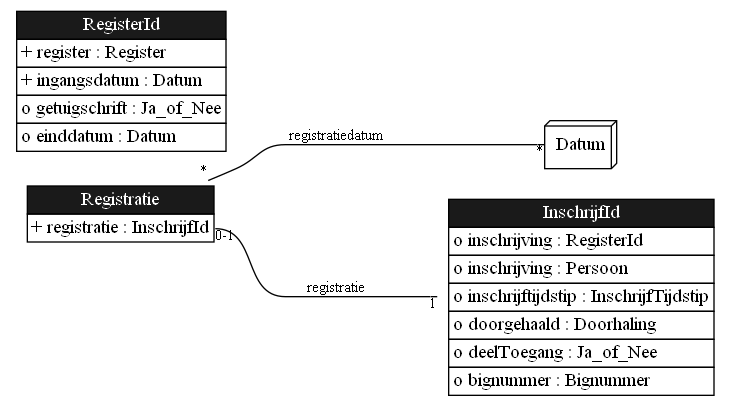
\includegraphics{C:/Users/gerar/OneDrive/OU/master/SE graduation/uitvoering/pattern/docs/images/CDPatternRegistratie.dot}
\caption{Figuur 4.5: Conceptueel diagram van
Registratie}\label{fig:Conceptueelux20diagramux20vanux20Registratie}
}
\end{figure}

\begin{longtable}[]{@{}ll@{}}
\toprule
Relatie & Betekenis \\
\midrule
\endhead
registratie {[}Registratie*InschrijfId{]} & \\
registratiedatum {[}Registratie*Datum{]} & \\
\bottomrule
\end{longtable}

\hypertarget{sec:SharedLangtheme-511868836}{%
\section{Inschrijving}\label{sec:SharedLangtheme-511868836}}

Inschrijving legt de relatie vast tussen Persoon en het Register.

In artikel 3 lid 2 wordt aangegeven dat bij elke inschrijving worden in
het register vermeld de naam, voornamen, geslacht, geboortedatum,
nationaliteit en adres van de betrokkene en het nummer en het tijdstip
van inschrijving. Bij ministeriële regeling kunnen gegevens worden
aangewezen die ten behoeve van het identificeren van beroepsbeoefenaren
bij de inschrijving worden vermeld.

\begin{description}
\tightlist
\item[Definitie 4:]
De aanmelding van persoon in een register
\end{description}

In artikel 3 lid 2 is aangegeven dat de datum en het tijdstip van
inschrijving een onderdeel is van de identificatie van de zorgverlener.

\begin{description}
\tightlist
\item[Definitie 5:]
Het inschrijftijdstip bevat de datum en tijdstip van inschrijving in
Y-m-d h:i:s-formaat.
\end{description}

In artikel 3 lid 2 wordt aangegeven dat bij elke inschrijving in het
register de naam, voornamen, geslacht, geboortedatum, nationaliteit en
adres van de betrokkene en het nummer en het tijdstip van inschrijving
wordt vermeld. Bij ministeriële regeling kunnen gegevens worden
aangewezen die ten behoeve van het identificeren van beroepsbeoefenaren
bij de inschrijving worden vermeld. Het BIG-nummer identificeert de
BIG-ingeschrevene.

\begin{description}
\tightlist
\item[Definitie 6:]
Het identificatienummer van de BIG-ingeschrevene.
\end{description}

4.6 Conceptueel diagram van ‘Inschrijving’.

\begin{figure}
\hypertarget{fig:Conceptueelux20diagramux20vanux20Inschrijving}{%
\centering
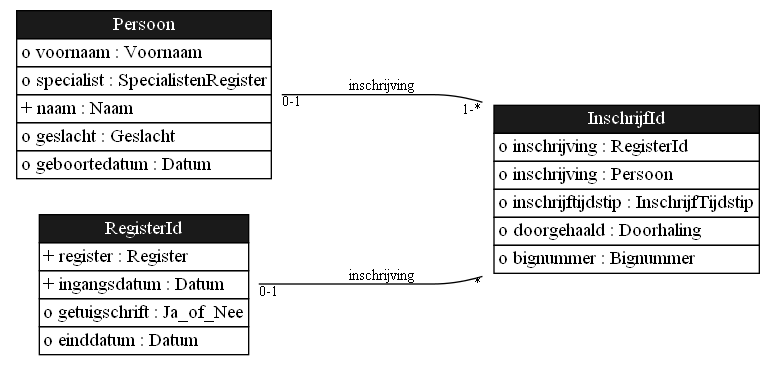
\includegraphics{C:/Users/gerar/OneDrive/OU/master/SE graduation/uitvoering/pattern/docs/images/CDPatternInschrijving.dot}
\caption{Figuur 4.6: Conceptueel diagram van
Inschrijving}\label{fig:Conceptueelux20diagramux20vanux20Inschrijving}
}
\end{figure}

\subsection{InschrijfId}

\begin{longtable}[]{@{}ll@{}}
\toprule
Attribuut & Betekenis \\
\midrule
\endhead
inschrijving & Het vastleggen van de koppeling tussen het register en de
inschrijving. \\
inschrijving & Elk persoon die BIG geregistreerd wil zijn, moet zijn
ingeschreven. Een persoon kan meerdere inschrijvingen hebben. \\
inschrijftijdstip & Elke inschrijving vindt plaats op een tijdstip. \\
\bottomrule
\end{longtable}

\begin{longtable}[]{@{}ll@{}}
\toprule
Relatie & Betekenis \\
\midrule
\endhead
bignummer {[}InschrijfId*Bignummer{]} & De koppeling tussen een Persoon
en een Bignummer. Dit is een één op één koppeling die automatisch wordt
aangebracht. \\
\bottomrule
\end{longtable}

\hypertarget{sec:SharedLangtheme--794606777}{%
\section{Register}\label{sec:SharedLangtheme--794606777}}

Het BIG-register (Beroepen in de Individuele Gezondheidszorg) is een
wettelijk, online en openbaar register. Alleen wie in het BIG-register
staat, mag een beschermde beroepstitel voeren en mag de bij het beroep
horende voorbehouden handelingen zelfstandig uitvoeren. Iedereen kan het
register raadplegen. Het BIG-register verzorgt ook de erkenning van
buitenlandse diploma’s.

\begin{description}
\tightlist
\item[Definitie 7:]
Technisch element voor het register.
\end{description}

In artikel 1 lid 5 wordt aangegeven dat elk Register wordt ingesteld en
beheerd door Onze Minister. In artikel 3 lid 6 wordt gesteld dat de
registers worden ingesteld ten einde te kunnen voldoen aan een verzoek
om informatie als bedoeld in artikel 12 en ten behoeve van het toezicht
op de uitvoering van de artikelen 4 en 17.

\begin{description}
\tightlist
\item[Definitie 8:]
Een register is een officiele lijst van personen die aan de, door het
register gestelde voorwaarden voldoen.
\end{description}

4.7 Conceptueel diagram van ‘Register’.

\begin{figure}
\hypertarget{fig:Conceptueelux20diagramux20vanux20Register}{%
\centering
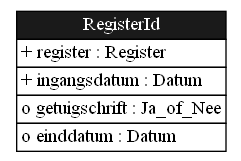
\includegraphics{C:/Users/gerar/OneDrive/OU/master/SE graduation/uitvoering/pattern/docs/images/CDPatternRegister.dot}
\caption{Figuur 4.7: Conceptueel diagram van
Register}\label{fig:Conceptueelux20diagramux20vanux20Register}
}
\end{figure}

\begin{longtable}[]{@{}ll@{}}
\toprule
Relatie & Betekenis \\
\midrule
\endhead
einddatum {[}RegisterId*Datum{]} & \\
getuigschrift {[}RegisterId*Ja\_of\_Nee{]} & \\
ingangsdatum {[}RegisterId*Datum{]} & \\
register {[}RegisterId*Register{]} & \\
\bottomrule
\end{longtable}

\hypertarget{sec:SharedLangtheme-1128353840}{%
\section{Arts}\label{sec:SharedLangtheme-1128353840}}

Het register voor arts bevat alle attributen van het register arts.

4.8 Conceptueel diagram van ‘Arts’.

\begin{figure}
\hypertarget{fig:Conceptueelux20diagramux20vanux20Arts}{%
\centering
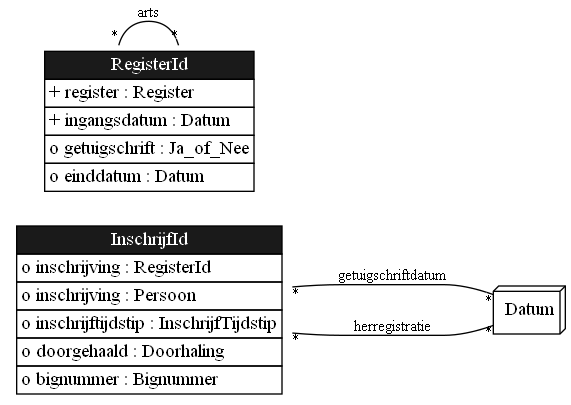
\includegraphics{C:/Users/gerar/OneDrive/OU/master/SE graduation/uitvoering/pattern/docs/images/CDPatternArts.dot}
\caption{Figuur 4.8: Conceptueel diagram van
Arts}\label{fig:Conceptueelux20diagramux20vanux20Arts}
}
\end{figure}

\begin{longtable}[]{@{}
  >{\raggedright\arraybackslash}p{(\columnwidth - 2\tabcolsep) * \real{0.50}}
  >{\raggedright\arraybackslash}p{(\columnwidth - 2\tabcolsep) * \real{0.50}}@{}}
\toprule
Relatie & Betekenis \\
\midrule
\endhead
arts {[}RegisterId*RegisterId{]} & \\
getuigschriftdatum {[}InschrijfId*Datum{]} & Er is een getuigschrift bij
een inschrijving geregistreerd dat relevant is voor het bepalen van de
geldigheid van die inschrijving.

Een register registreert datum waarop de ingeschrevene een bij of
krachtens hoofdstuk III of VI aangewezen getuigschrift heeft verkregen,
zoals bedoeld in Art. 8 lid 2 sub a van de Wet BIG. Als er meerdere
getuigschriften zijn, kunnen er dus ook meerdere data zijn bij dezelfde
inschrijving.

Een register registreert datum waarop de ingeschrevene een bij of
krachtens hoofdstuk III of VI aangewezen getuigschrift heeft verkregen,
zoals bedoeld in Art. 8 lid 2 sub a van de Wet BIG. Als er meerdere
getuigschriften zijn, kunnen er dus ook meerdere data zijn bij dezelfde
inschrijving.

Een register registreert datum waarop de ingeschrevene een bij of
krachtens hoofdstuk III of VI aangewezen getuigschrift heeft verkregen,
zoals bedoeld in Art. 8 lid 2 sub a van de Wet BIG. Als er meerdere
getuigschriften zijn, kunnen er dus ook meerdere data zijn bij dezelfde
inschrijving.

Een register registreert datum waarop de ingeschrevene een bij of
krachtens hoofdstuk III of VI aangewezen getuigschrift heeft verkregen,
zoals bedoeld in Art. 8 lid 2 sub a van de Wet BIG. Als er meerdere
getuigschriften zijn, kunnen er dus ook meerdere data zijn bij dezelfde
inschrijving. \\
herregistratie {[}InschrijfId*Datum{]} & Artikel 2, tweede lid van het
Besluit periodieke registratie Wet Big stelt dat de datum van
herregistratie op vijf jaar na datum van registratie. \\
\bottomrule
\end{longtable}

\hypertarget{sec:SharedLangtheme-1982034445}{%
\section{Tandarts}\label{sec:SharedLangtheme-1982034445}}

Het register voor tandarts bevat alle attributen van het register
tandarts.

4.9 Conceptueel diagram van ‘Tandarts’.

\begin{figure}
\hypertarget{fig:Conceptueelux20diagramux20vanux20Tandarts}{%
\centering
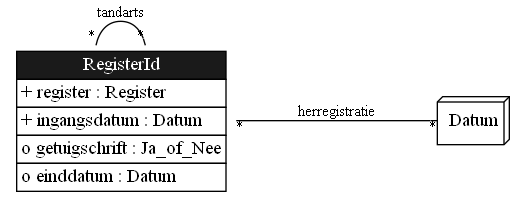
\includegraphics{C:/Users/gerar/OneDrive/OU/master/SE graduation/uitvoering/pattern/docs/images/CDPatternTandarts.dot}
\caption{Figuur 4.9: Conceptueel diagram van
Tandarts}\label{fig:Conceptueelux20diagramux20vanux20Tandarts}
}
\end{figure}

\begin{longtable}[]{@{}
  >{\raggedright\arraybackslash}p{(\columnwidth - 2\tabcolsep) * \real{0.50}}
  >{\raggedright\arraybackslash}p{(\columnwidth - 2\tabcolsep) * \real{0.50}}@{}}
\toprule
Relatie & Betekenis \\
\midrule
\endhead
getuigschriftdatum {[}InschrijfId*Datum{]} & Er is een getuigschrift bij
een inschrijving geregistreerd dat relevant is voor het bepalen van de
geldigheid van die inschrijving.

Een register registreert datum waarop de ingeschrevene een bij of
krachtens hoofdstuk III of VI aangewezen getuigschrift heeft verkregen,
zoals bedoeld in Art. 8 lid 2 sub a van de Wet BIG. Als er meerdere
getuigschriften zijn, kunnen er dus ook meerdere data zijn bij dezelfde
inschrijving.

Een register registreert datum waarop de ingeschrevene een bij of
krachtens hoofdstuk III of VI aangewezen getuigschrift heeft verkregen,
zoals bedoeld in Art. 8 lid 2 sub a van de Wet BIG. Als er meerdere
getuigschriften zijn, kunnen er dus ook meerdere data zijn bij dezelfde
inschrijving.

Een register registreert datum waarop de ingeschrevene een bij of
krachtens hoofdstuk III of VI aangewezen getuigschrift heeft verkregen,
zoals bedoeld in Art. 8 lid 2 sub a van de Wet BIG. Als er meerdere
getuigschriften zijn, kunnen er dus ook meerdere data zijn bij dezelfde
inschrijving.

Een register registreert datum waarop de ingeschrevene een bij of
krachtens hoofdstuk III of VI aangewezen getuigschrift heeft verkregen,
zoals bedoeld in Art. 8 lid 2 sub a van de Wet BIG. Als er meerdere
getuigschriften zijn, kunnen er dus ook meerdere data zijn bij dezelfde
inschrijving. \\
herregistratie {[}RegisterId*Datum{]} & Artikel 2, tweede lid van het
Besluit periodieke registratie Wet Big stelt dat de datum van
herregistratie op vijf jaar na datum van registratie. \\
tandarts {[}RegisterId*RegisterId{]} & \\
\bottomrule
\end{longtable}

\hypertarget{sec:SharedLangtheme--231419835}{%
\section{Apotheker}\label{sec:SharedLangtheme--231419835}}

Het register voor tandarts bevat alle attributen van het register
tandarts.

4.10 Conceptueel diagram van ‘Apotheker’.

\begin{figure}
\hypertarget{fig:Conceptueelux20diagramux20vanux20Apotheker}{%
\centering
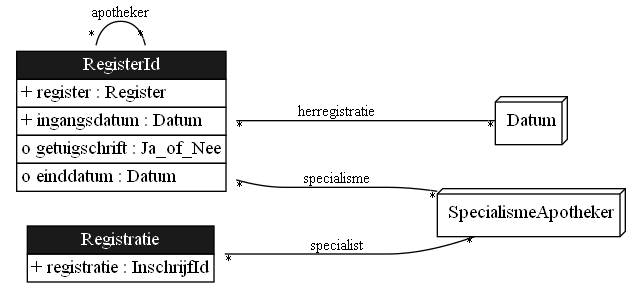
\includegraphics{C:/Users/gerar/OneDrive/OU/master/SE graduation/uitvoering/pattern/docs/images/CDPatternApotheker.dot}
\caption{Figuur 4.10: Conceptueel diagram van
Apotheker}\label{fig:Conceptueelux20diagramux20vanux20Apotheker}
}
\end{figure}

\begin{longtable}[]{@{}
  >{\raggedright\arraybackslash}p{(\columnwidth - 2\tabcolsep) * \real{0.50}}
  >{\raggedright\arraybackslash}p{(\columnwidth - 2\tabcolsep) * \real{0.50}}@{}}
\toprule
Relatie & Betekenis \\
\midrule
\endhead
apotheker {[}RegisterId*RegisterId{]} & \\
getuigschriftdatum {[}InschrijfId*Datum{]} & Er is een getuigschrift bij
een inschrijving geregistreerd dat relevant is voor het bepalen van de
geldigheid van die inschrijving.

Een register registreert datum waarop de ingeschrevene een bij of
krachtens hoofdstuk III of VI aangewezen getuigschrift heeft verkregen,
zoals bedoeld in Art. 8 lid 2 sub a van de Wet BIG. Als er meerdere
getuigschriften zijn, kunnen er dus ook meerdere data zijn bij dezelfde
inschrijving.

Een register registreert datum waarop de ingeschrevene een bij of
krachtens hoofdstuk III of VI aangewezen getuigschrift heeft verkregen,
zoals bedoeld in Art. 8 lid 2 sub a van de Wet BIG. Als er meerdere
getuigschriften zijn, kunnen er dus ook meerdere data zijn bij dezelfde
inschrijving.

Een register registreert datum waarop de ingeschrevene een bij of
krachtens hoofdstuk III of VI aangewezen getuigschrift heeft verkregen,
zoals bedoeld in Art. 8 lid 2 sub a van de Wet BIG. Als er meerdere
getuigschriften zijn, kunnen er dus ook meerdere data zijn bij dezelfde
inschrijving.

Een register registreert datum waarop de ingeschrevene een bij of
krachtens hoofdstuk III of VI aangewezen getuigschrift heeft verkregen,
zoals bedoeld in Art. 8 lid 2 sub a van de Wet BIG. Als er meerdere
getuigschriften zijn, kunnen er dus ook meerdere data zijn bij dezelfde
inschrijving. \\
herregistratie {[}RegisterId*Datum{]} & Artikel 2, tweede lid van het
Besluit periodieke registratie Wet Big stelt dat de datum van
herregistratie op vijf jaar na datum van registratie. \\
\bottomrule
\end{longtable}

\hypertarget{sec:SharedLangtheme-1761117493}{%
\section{Geslacht}\label{sec:SharedLangtheme-1761117493}}

In Artikel 3 lid 2 is bepaald dat het geslacht van de inschrijver een
onderdeel is van de identificatie van de zorgverlener.

\begin{description}
\tightlist
\item[Definitie 9:]
De sekse van een individue.
\end{description}

Nadere duiding van de afkorting die gebruik wordt voor geslacht.

\begin{description}
\tightlist
\item[Definitie 10:]
Omschrijving van het geslacht van een individue.
\end{description}

4.11 Conceptueel diagram van ‘Geslacht’.

\begin{figure}
\hypertarget{fig:Conceptueelux20diagramux20vanux20Geslacht}{%
\centering
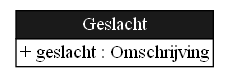
\includegraphics{C:/Users/gerar/OneDrive/OU/master/SE graduation/uitvoering/pattern/docs/images/CDPatternGeslacht.dot}
\caption{Figuur 4.11: Conceptueel diagram van
Geslacht}\label{fig:Conceptueelux20diagramux20vanux20Geslacht}
}
\end{figure}

\begin{longtable}[]{@{}ll@{}}
\toprule
Relatie & Betekenis \\
\midrule
\endhead
geslacht {[}Geslacht*Omschrijving{]} & \\
\bottomrule
\end{longtable}

\hypertarget{sec:SharedLangtheme--42209667}{%
\section{Nationaliteit}\label{sec:SharedLangtheme--42209667}}

Nationaliteit duidt de relatie aan tussen een individu en een staat.

In artikel 3 lid 2 is aangegeven dat de Nationaliteit van de betrokkene
bij Inschrijving moet worden vermeld, als onderdeel van de identificatie
van de zorgverlener.

\begin{description}
\tightlist
\item[Definitie 11:]
De Nationaliteit wordt aangeduid middels een 4-cijferige code.
\end{description}

Door een omschrijving toe te voegen wordt de nationaliteitcodering
leesbaar.

\begin{description}
\tightlist
\item[Definitie 12:]
De omschrijving van een nationaliteit bevat de tekstuele uitvoering van
de nationaliteitscodering.
\end{description}

4.12 Conceptueel diagram van ‘Nationaliteit’.

\begin{figure}
\hypertarget{fig:Conceptueelux20diagramux20vanux20Nationaliteit}{%
\centering
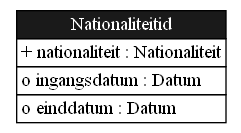
\includegraphics{C:/Users/gerar/OneDrive/OU/master/SE graduation/uitvoering/pattern/docs/images/CDPatternNationaliteit.dot}
\caption{Figuur 4.12: Conceptueel diagram van
Nationaliteit}\label{fig:Conceptueelux20diagramux20vanux20Nationaliteit}
}
\end{figure}

\subsection{Nationaliteitid}

\begin{longtable}[]{@{}ll@{}}
\toprule
Attribuut & Betekenis \\
\midrule
\endhead
nationaliteit & Het aanbrengen van de koppeling tussen de
nationaliteitcode en de bijbehorende omschrijving. Bij elke code hoort
maar één omschrijving en de omschrijving behoort maar tot één code. \\
ingangsdatum & Ingangsdatum van de Nationaliteit. \\
einddatum & Einddatum van gebruik van de Nationaliteit. \\
\bottomrule
\end{longtable}

\begin{longtable}[]{@{}ll@{}}
\toprule
Relatie & Betekenis \\
\midrule
\endhead
\bottomrule
\end{longtable}

\hypertarget{sec:SharedLangtheme-326791551}{%
\section{Adres}\label{sec:SharedLangtheme-326791551}}

In artikel 3 lid 2 is aangegeven dat het adres een onderdeel is van de
identificatie van de zorgverlener.

\begin{description}
\tightlist
\item[Definitie 13:]
Bevat het adres van de Persoon zoals vastgelegd binnen de BRP.
\end{description}

\begin{description}
\tightlist
\item[Definitie 14:]
\end{description}

\begin{description}
\tightlist
\item[Definitie 15:]
\end{description}

4.13 Conceptueel diagram van ‘Adres’.

\begin{figure}
\hypertarget{fig:Conceptueelux20diagramux20vanux20Adres}{%
\centering
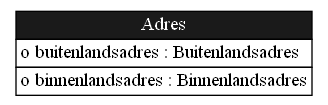
\includegraphics{C:/Users/gerar/OneDrive/OU/master/SE graduation/uitvoering/pattern/docs/images/CDPatternAdres.dot}
\caption{Figuur 4.13: Conceptueel diagram van
Adres}\label{fig:Conceptueelux20diagramux20vanux20Adres}
}
\end{figure}

\begin{longtable}[]{@{}ll@{}}
\toprule
Relatie & Betekenis \\
\midrule
\endhead
binnenlandsadres {[}Adres*Binnenlandsadres{]} & \\
buitenlandsadres {[}Adres*Buitenlandsadres{]} & \\
\bottomrule
\end{longtable}

\hypertarget{sec:SharedLangtheme-949118634}{%
\section{Persoon}\label{sec:SharedLangtheme-949118634}}

In artikel 3 lid 2 wordt aangegeven dat bij elke inschrijving in het
register de naam, voornamen, geslacht, geboortedatum, nationaliteit en
adres van de betrokkene en het nummer en het tijdstip van inschrijving
wordt vermeld. Bij ministeriële regeling kunnen gegevens worden
aangewezen die ten behoeve van het identificeren van beroepsbeoefenaren
bij de inschrijving worden vermeld. Deze beroepsbeoefenaren zijn
personen.

\begin{description}
\tightlist
\item[Definitie 16:]
Een Persoon representeerd een persoons-id dat opgenomen is in het
BIG-register.
\end{description}

In artikel 3 lid 2 is aangegeven dat de naam een onderdeel is van de
identificatie van de zorgverlener.

\begin{description}
\tightlist
\item[Definitie 17:]
Aanduiding van de familienaam zoals vastgelegd in de BRP.
\end{description}

In artikel 3 lid 2 is aangegeven dat de voorna(a)m(en) een onderdeel
is/zijn van de identificatie van de zorgverlener.

\begin{description}
\tightlist
\item[Definitie 18:]
Alle voornamen van de Persoon zoals dit is vastgelegd binnen de BRP.
\end{description}

4.14 Conceptueel diagram van ‘Persoon’.

\begin{figure}
\hypertarget{fig:Conceptueelux20diagramux20vanux20Persoon}{%
\centering
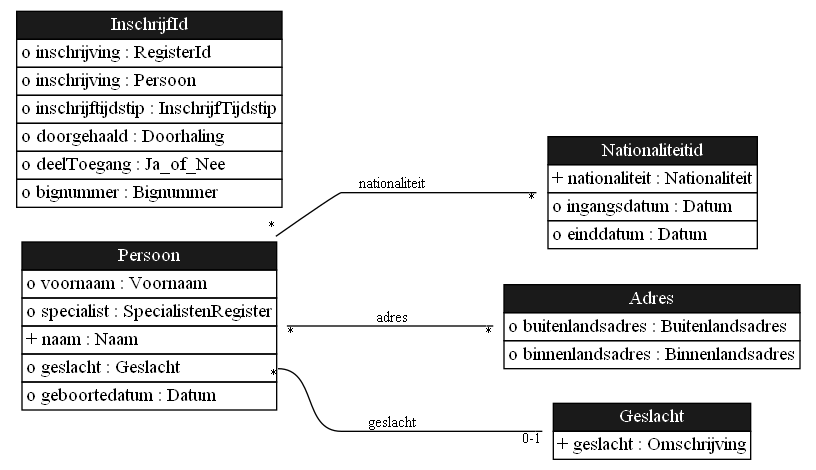
\includegraphics{C:/Users/gerar/OneDrive/OU/master/SE graduation/uitvoering/pattern/docs/images/CDPatternPersoon.dot}
\caption{Figuur 4.14: Conceptueel diagram van
Persoon}\label{fig:Conceptueelux20diagramux20vanux20Persoon}
}
\end{figure}

\subsection{Persoon}

\begin{longtable}[]{@{}ll@{}}
\toprule
Attribuut & Betekenis \\
\midrule
\endhead
voornaam & Elke ingeschrevene moet een voornaam hebben. \\
naam & Elke ingeschrevene moet een naam hebben en een naam kan bij
meerdere personen behoren. \\
geslacht & Elke ingeschrevene behoort tot een geslacht \\
geboortedatum & Elke ingeschrevene heeft een geboortedatum \\
\bottomrule
\end{longtable}

\begin{longtable}[]{@{}ll@{}}
\toprule
Relatie & Betekenis \\
\midrule
\endhead
adres {[}Persoon*Adres{]} & Elke ingeschrevene heeft een adres \\
nationaliteit {[}Persoon*Nationaliteitid{]} & Elke ingeschrevene heeft
een nationaliteit \\
\bottomrule
\end{longtable}

\hypertarget{sec:SharedLangtheme--1935921574}{%
\section{Overig}\label{sec:SharedLangtheme--1935921574}}

\begin{description}
\tightlist
\item[Definitie 19:]
\end{description}

\begin{description}
\tightlist
\item[Definitie 20:]
description
\end{description}

In Artikel 7 wordt beschreven in welke situatie de inschrijving wordt
doorgehaald:

\begin{enumerate}
\tightlist
\item
  in geval van overlijden van de ingeschrevene;
\item
  op verzoek van de ingeschrevene;
\item
  indien de ingeschrevene in een der in artikel 6, onder b of c,
  genoemde omstandigheden is komen te verkeren;
\item
  indien zulks voortvloeit uit een op grond van deze wet jegens de
  ingeschrevene genomen maatregel;
\item
  indien ten aanzien van de ingeschrevene een maatregel, berustende op
  een in het buitenland gegeven rechterlijke, tuchtrechtelijke of
  bestuursrechtelijke beslissing van kracht is, op grond waarvan de
  ingeschrevene zijn rechten ter zake van de uitoefening van het
  betrokken beroep in het land waar de beslissing is gegeven tijdelijk
  of blijvend geheel heeft verloren;
\item
  indien zulks voortvloeit uit een maatregel, berustend op een op grond
  van de Wet medisch tuchtrecht BES opgelegde maatregel, op grond
  waarvan de ingeschrevene zijn rechten ter zake van de uitoefening van
  het betrokken beroep tijdelijk of blijvend geheel heeft verloren.
\end{enumerate}

\begin{description}
\tightlist
\item[Definitie 21:]
\end{description}

\begin{longtable}[]{@{}ll@{}}
\toprule
Relatie & Betekenis \\
\midrule
\endhead
doorgehaald {[}InschrijfId*Doorhaling{]} & In artikel 7 gestelde
sitatuaties waarin de inschrijving wordt doorgehaald. Deze heeft ook
consequenties op de bijbehorende registraties. \\
nietVerplicht {[}Ja\_of\_Nee*Ja\_of\_Nee{]} & \\
sessionToday {[}SESSION*Datum{]} & \\
verplicht {[}Ja\_of\_Nee*Ja\_of\_Nee{]} & \\
\bottomrule
\end{longtable}



\end{document}

